\chapter{System Development}


\section{System Architecture}

\begin{figure}
	\centering
	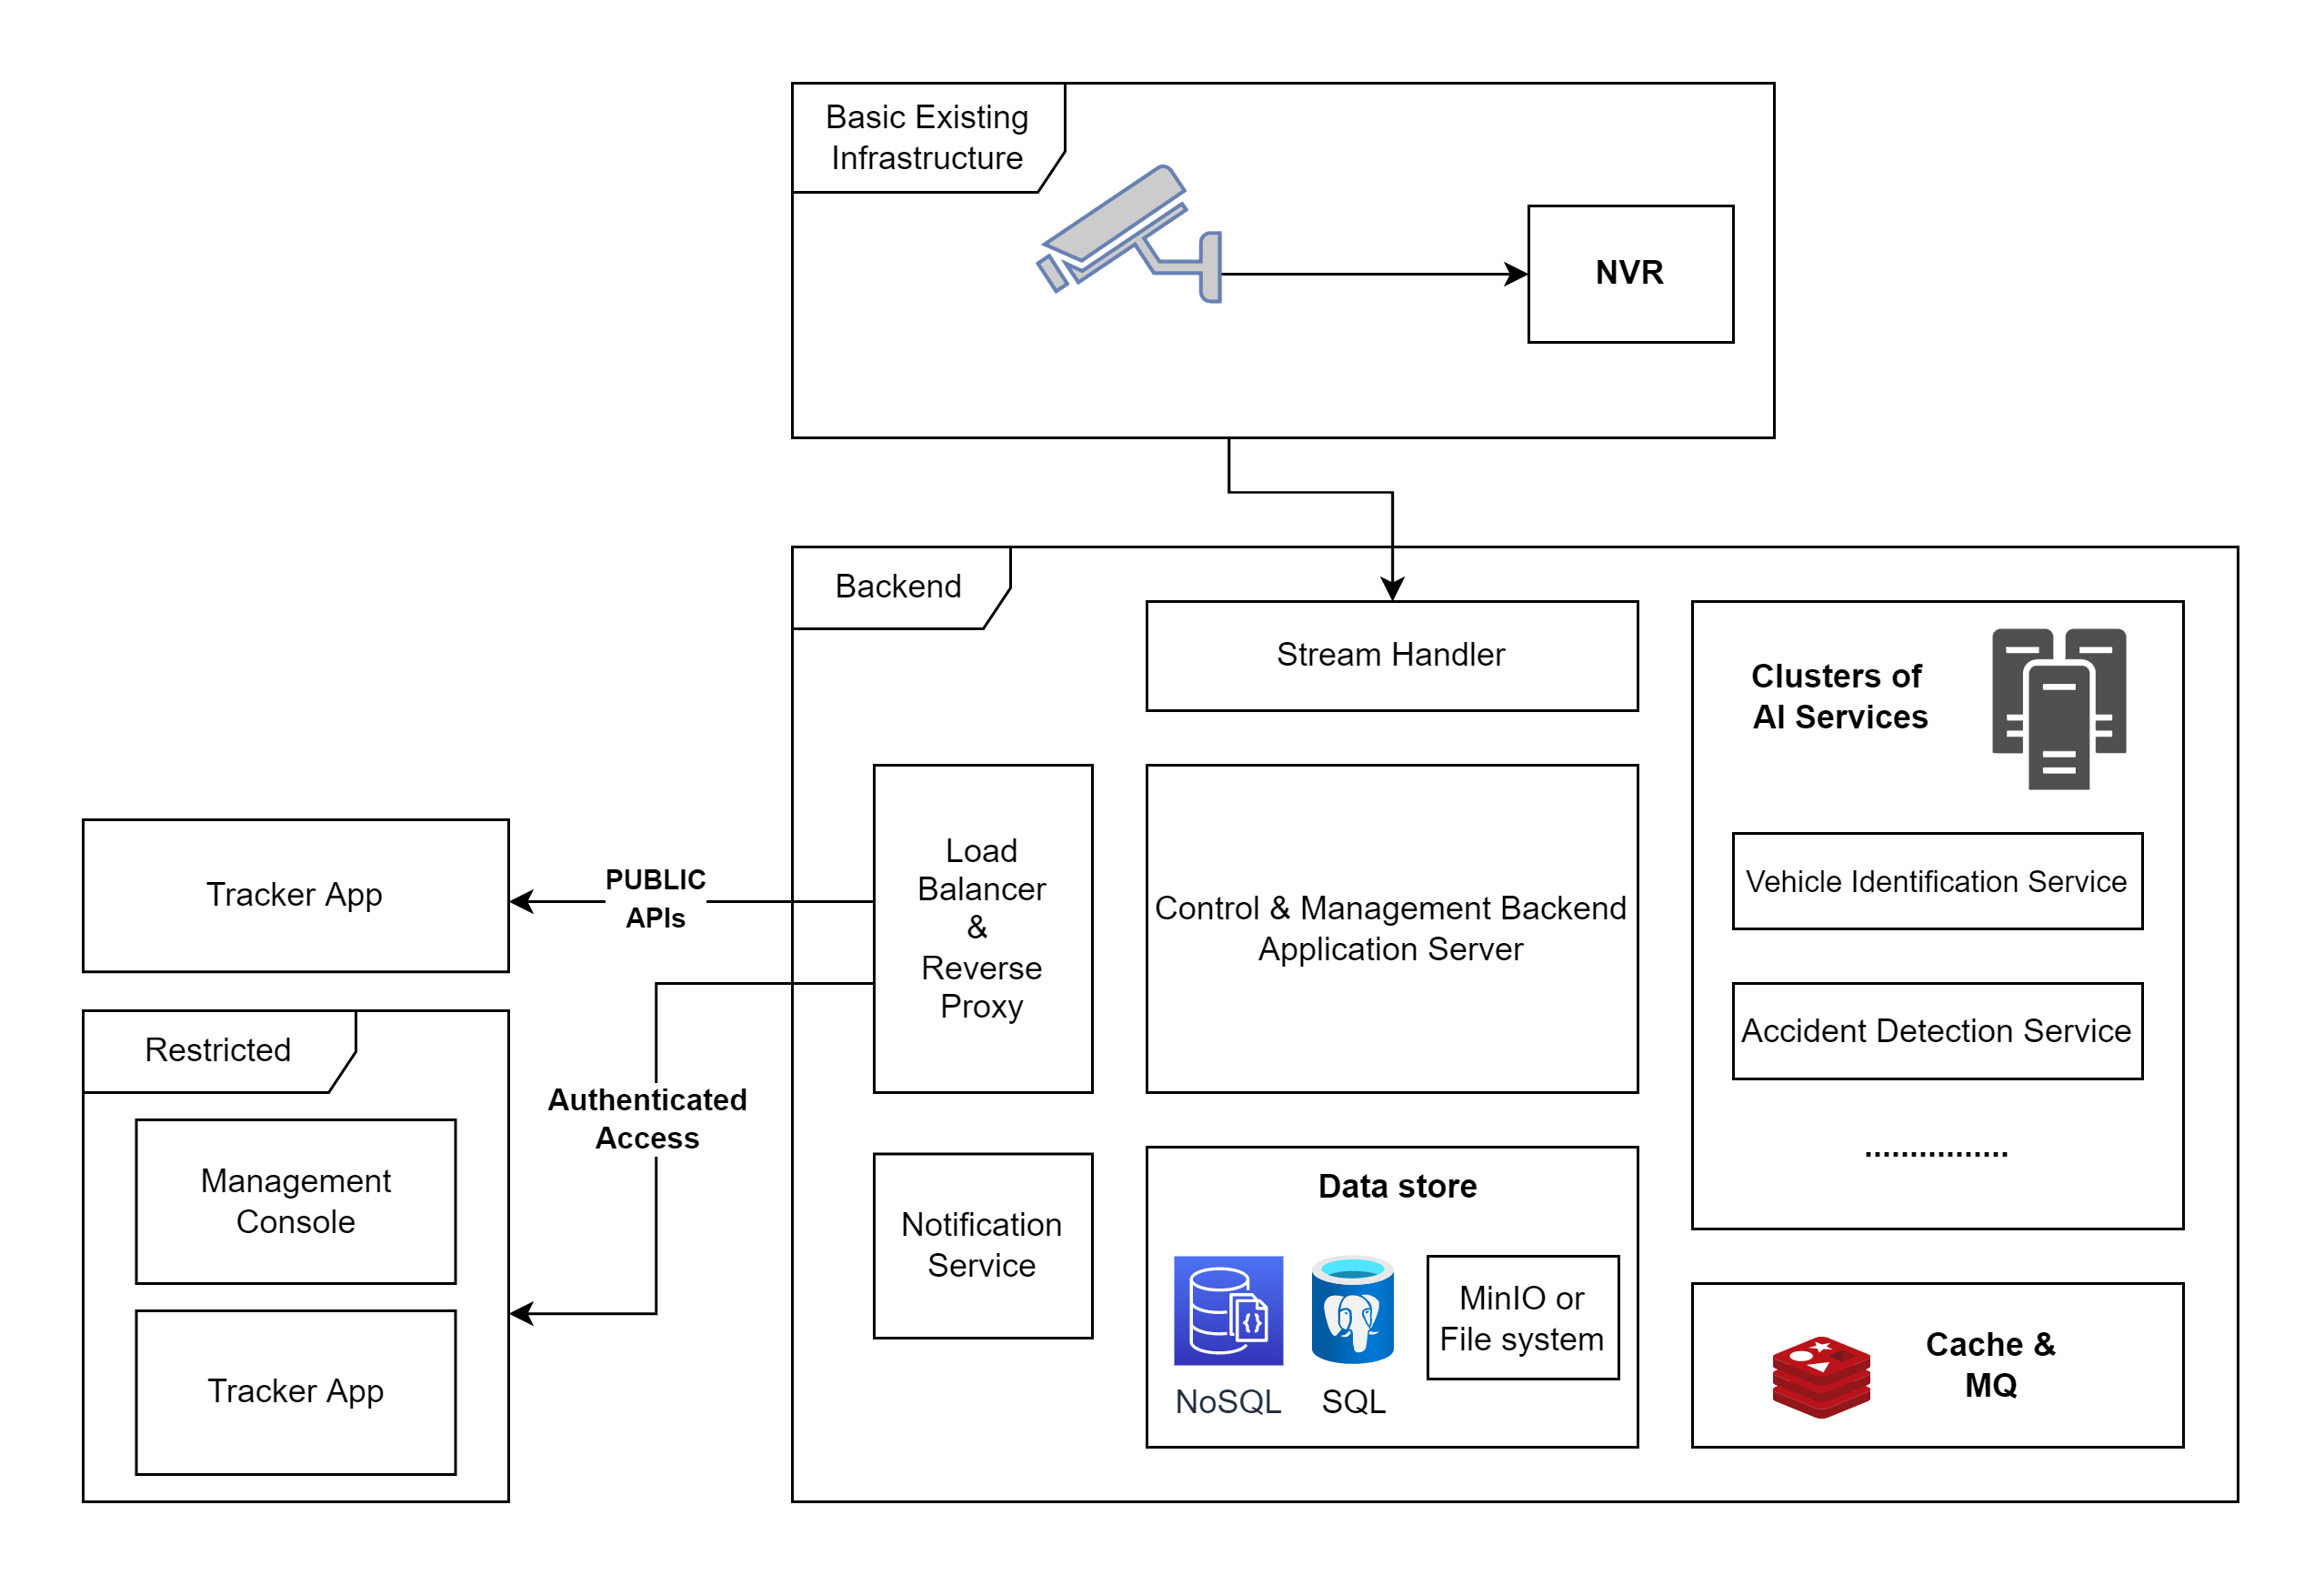
\includegraphics[width=0.8\linewidth]{Images/architecture_high_level}
	\caption{High level system architecture}
	\label{fig:architecturehighlevel}
\end{figure}


\subsection{Existing CCTV Infrastructure}
Modern Infrastructure of CCTV (Closed-Circuit Television) Video surveillance system pan out to a Network connected IP camera, which is streamed to an NVR (Network Video Recorder). Popular streaming protocols like RTSP (Realtime Streaming Protocol), RTSPS (RTSP over SSL), RTMP (Real-Time Messaging Protocol) are utilized in most IP cameras and NVR. 

NVR stores the footage and is usually removed after specified period based on the storage capacity of the NVR and number of cameras connected. On most NVR firmware, playback and downloading of recording is only provided by builtin web interface, or proprietary softwares bundled, which are known to be poorly implemented. Some NVR interface only works with full features on outdated Internet Explorer after installing plug-in.

Live streams of NVR and IP cameras can be accessed easily as RSTP stream using the network ip address, which can be played by any client in the same network.

\subsection{VPN based Secure network access}
CCTV Video surveillance systems utilize restricted closed network isolated from the internet, to reduce Cyber attack vectors and unauthorized usage. Unsecured connection and system usage can compromise the security of network. 
Constructing a VPN (Virtual Private Network) split tunnel can enable secure communication interface to the network over unsecured channels. Wireguard, distributed in Linux Kernel, is utilized in our design to create VPN interface with very less overhead and very high performance.

\subsection{Video Stream Ingestion}
Video stream from NVR and IP camera are ingested to our system by Stream Handler and FrameGen module for processing using OpenCV. FrameGen module reads the live stream of cameras specified and save frames to storage backend with timestamp and signature as metadata. It ignores dead frames, blacklisted and idle frames and saves only required frames thereby reducing storage requirement.

Additionally, FFmpeg is used for on-the-fly transcoding (transcoding while streaming) of live RSTP stream (which is a pull stream) from IP camera and NVR, to RTMP stream (which is a push stream) to NGINX Media Server. A stream key is attached to each stream which NGINX relays as HLS (HTTP Live Streaming) securely over SSL (Secure Socket Layer) to client browser of the authenticated user containing stream key.   

\subsection{Storage Backend}
For local development setup, Linux File system is used as storage backend. For production grade setup MinIO Server is used as the storage backend to provide secure redundancy, segregated access, and hybrid multi-tenant enterprise grade system. Each file is identified by the path and object id and can be retrieved by authorized users. 


\begin{figure}[ht!]
	\centering
	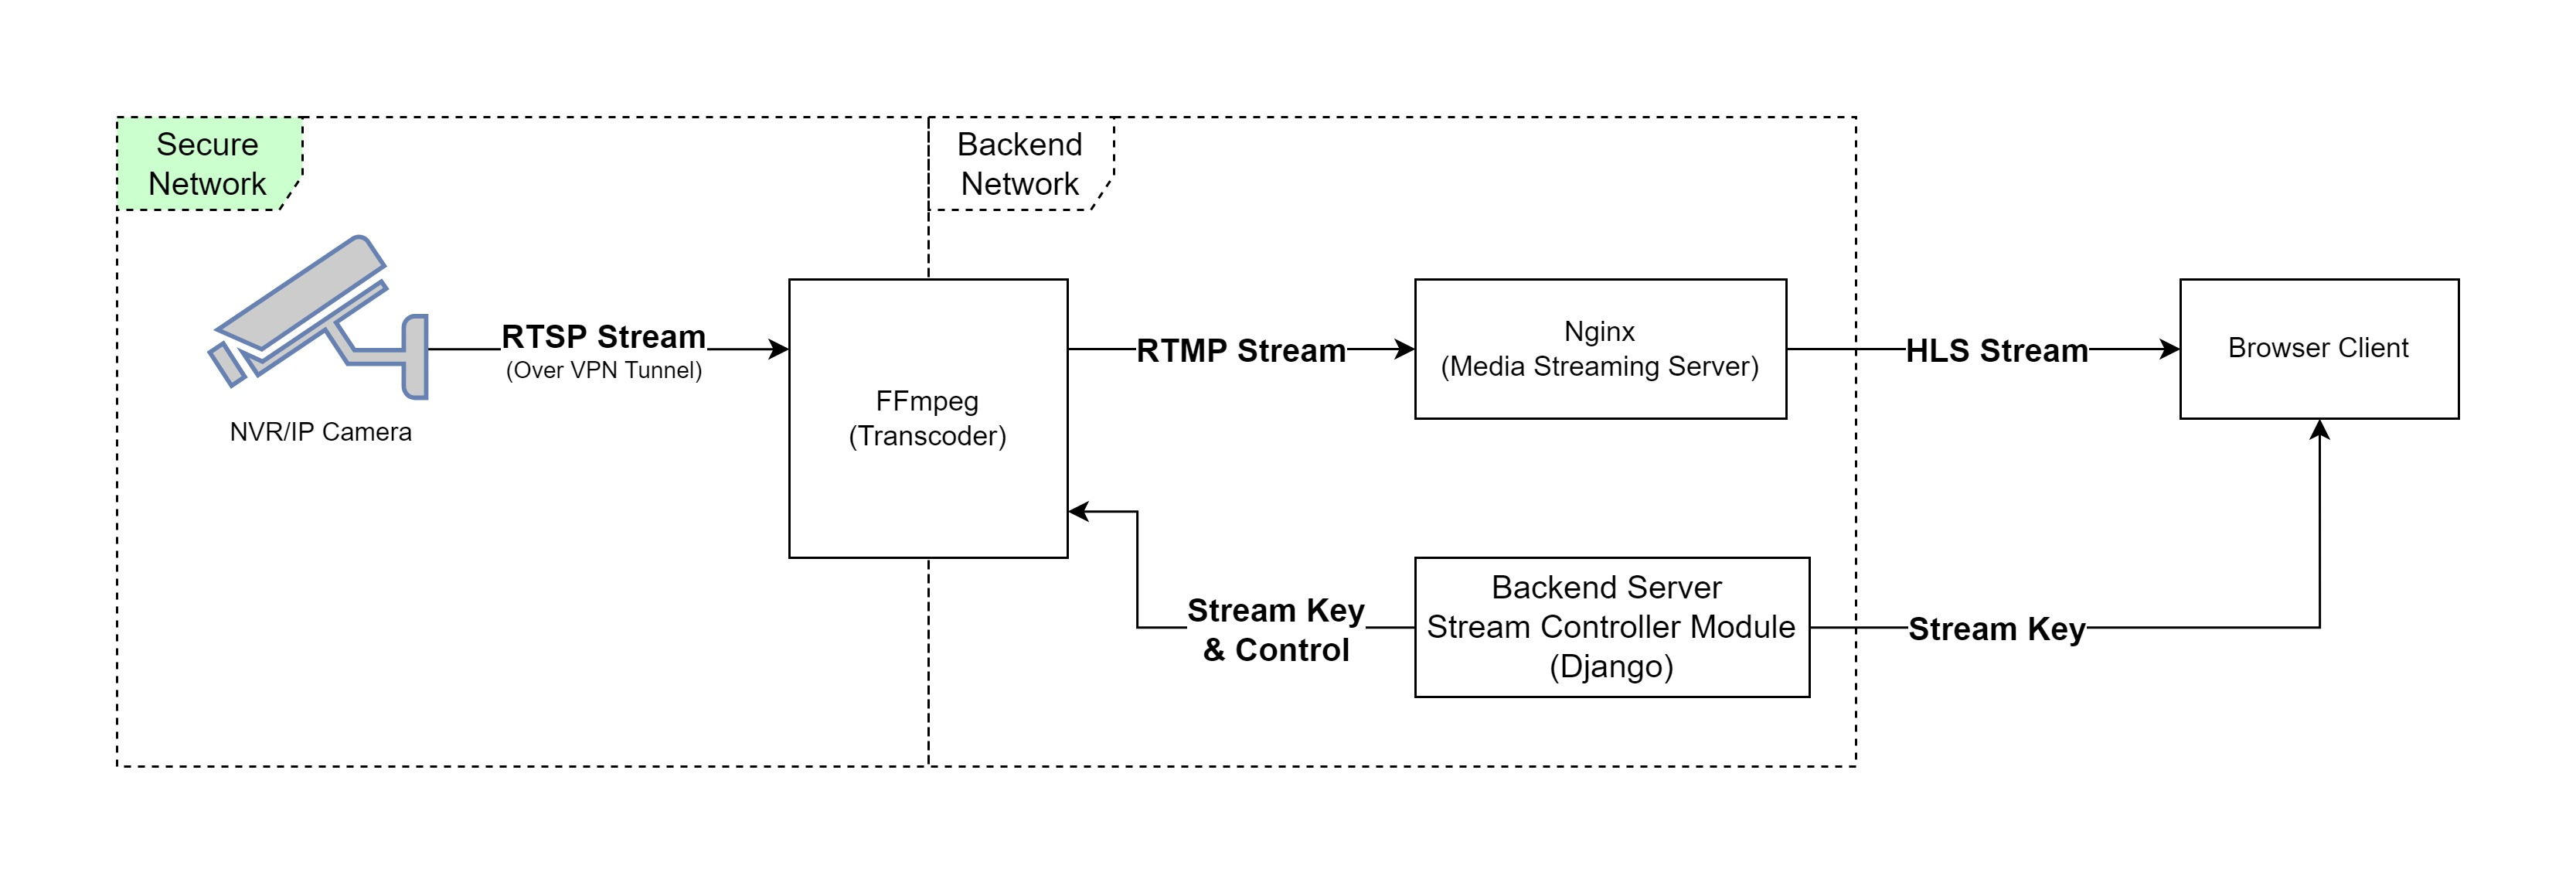
\includegraphics[width=0.8\linewidth]{Images/live_stream_arch}
	\caption{Camera Feed Live Streaming}
	\label{fig:livestreamarch}
\end{figure}

\subsection*{Technology Stack}
A hybrid microservice architecture is utilized to gain the scalability and decouple AI engine and services to serve web request efficiently, while ensuring quicker and simpler development and deployment. Each independent services are created as a separate modular microservice which can be integrated based on requirement and infrastructure availability.

Development is primarily done in Python, while JavaScript is utilized for front-end scripting.

The list of frameworks and libraries used represent those which are widely utilized or have significant impact in the development.

\subsubsection*{Languages}
\begin{itemize}
	\item Python (Primary Language): Used in all server-side code.
	\item JavaScript: Used in front-end Scripting, WebSocket Browser Client, OpenPlayerJS
\end{itemize}

\subsubsection*{Frameworks}
\begin{itemize}
	\item Django: Back-end Server
	\item FastAPI: API web framework for micro-service like AI Engine and provides WebSocket Abstraction
	\item Keras \& TensorFlow: AI inferencing
	\item Darknet \& CUDA: Training Model
\end{itemize}

\subsubsection*{Other Tools}
\begin{itemize}
	\item Nginx: Used as web server and reverse proxy for handling request, serving static files, proxying request to application servers.
	\item Nginx RTMP Module: Used to enhance Nginx to be used as a Media Streaming Server
	\item PostgreSQL: As Relational Database
	\item WireGaurd: Creating secured encrypted VPN tunnel to NVR infrastructure network
	\item FFmpeg: For on-the-fly video transcoding to relay Live Camera RSTP feed to nginx as RTMP ingress feed
	\item OpenCV: Image Processing in FrameGen module and handling camera feed.
	\item WebSocket: Bidirectional server-push communication with user
	\item OpenPlayerJS: Browser-based HLS video stream playback
	\item MinIO: File and object storage back-end to replicate Amazon Web Service S3.
	\item Docker: For containerisation of services
	\item GitHub Action: For Continous Integration and Deployment (CI/CD) pipleline
\end{itemize}


\begin{figure}[h!]
	\centering
	\begin{subfigure}[b]{0.8\linewidth}
		\centering
		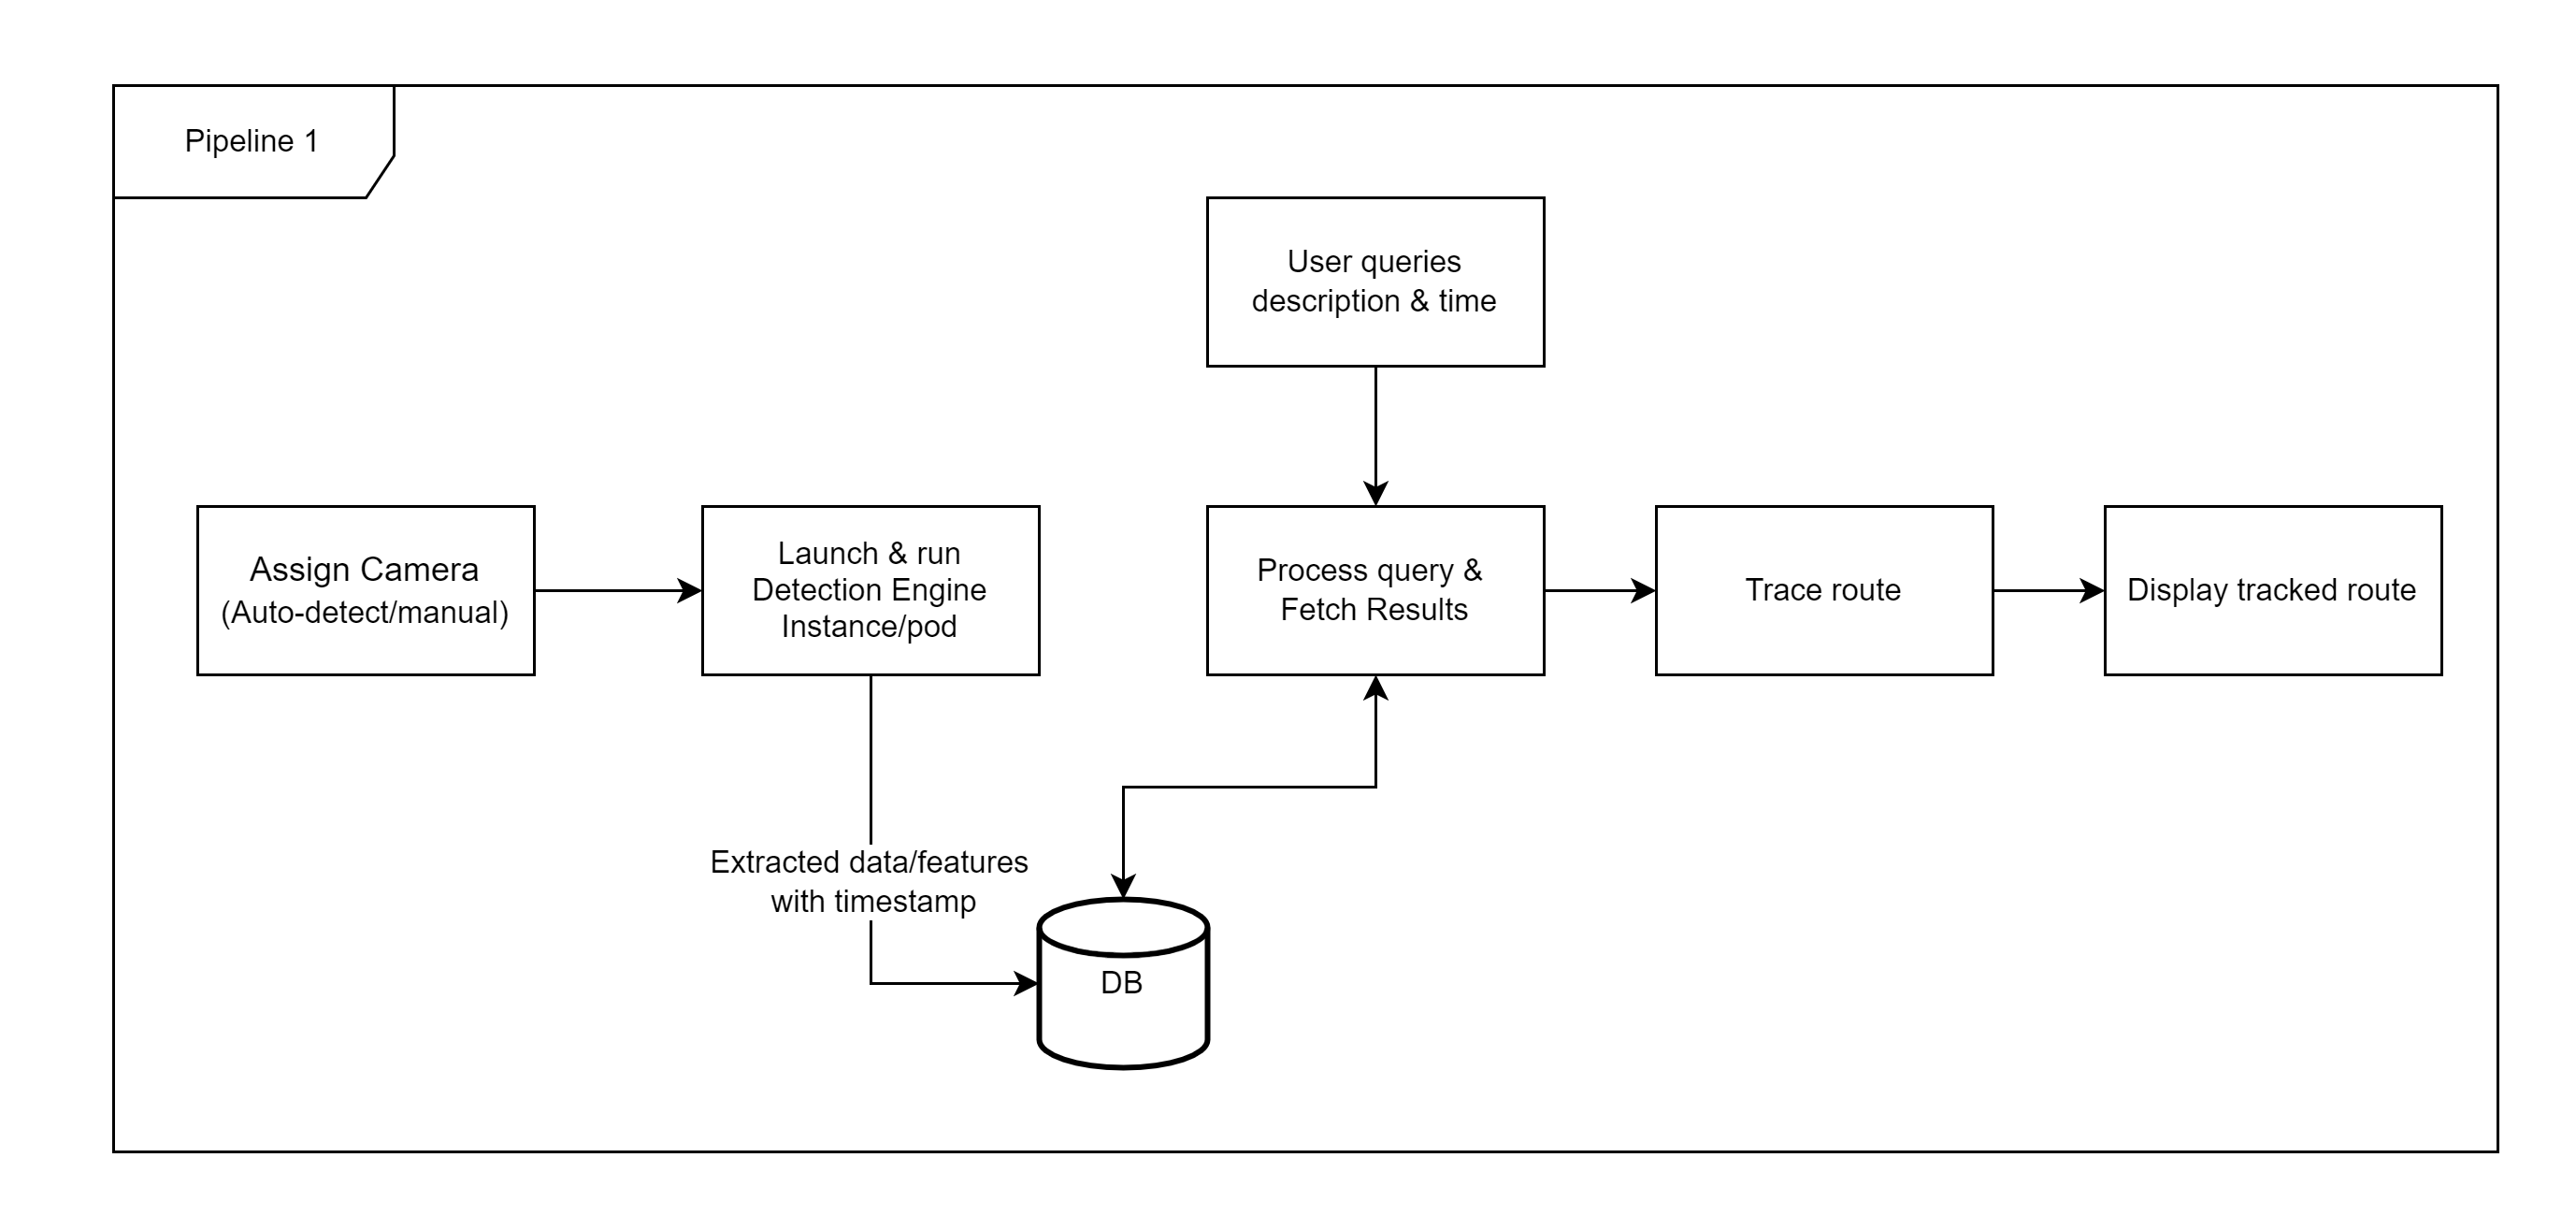
\includegraphics[width=\linewidth]{Images/pipeline1}
		\caption{pipeline1}
		\label{fig:pipeline1}
	\end{subfigure}

	\begin{subfigure}[b]{0.8\linewidth}
		\centering
		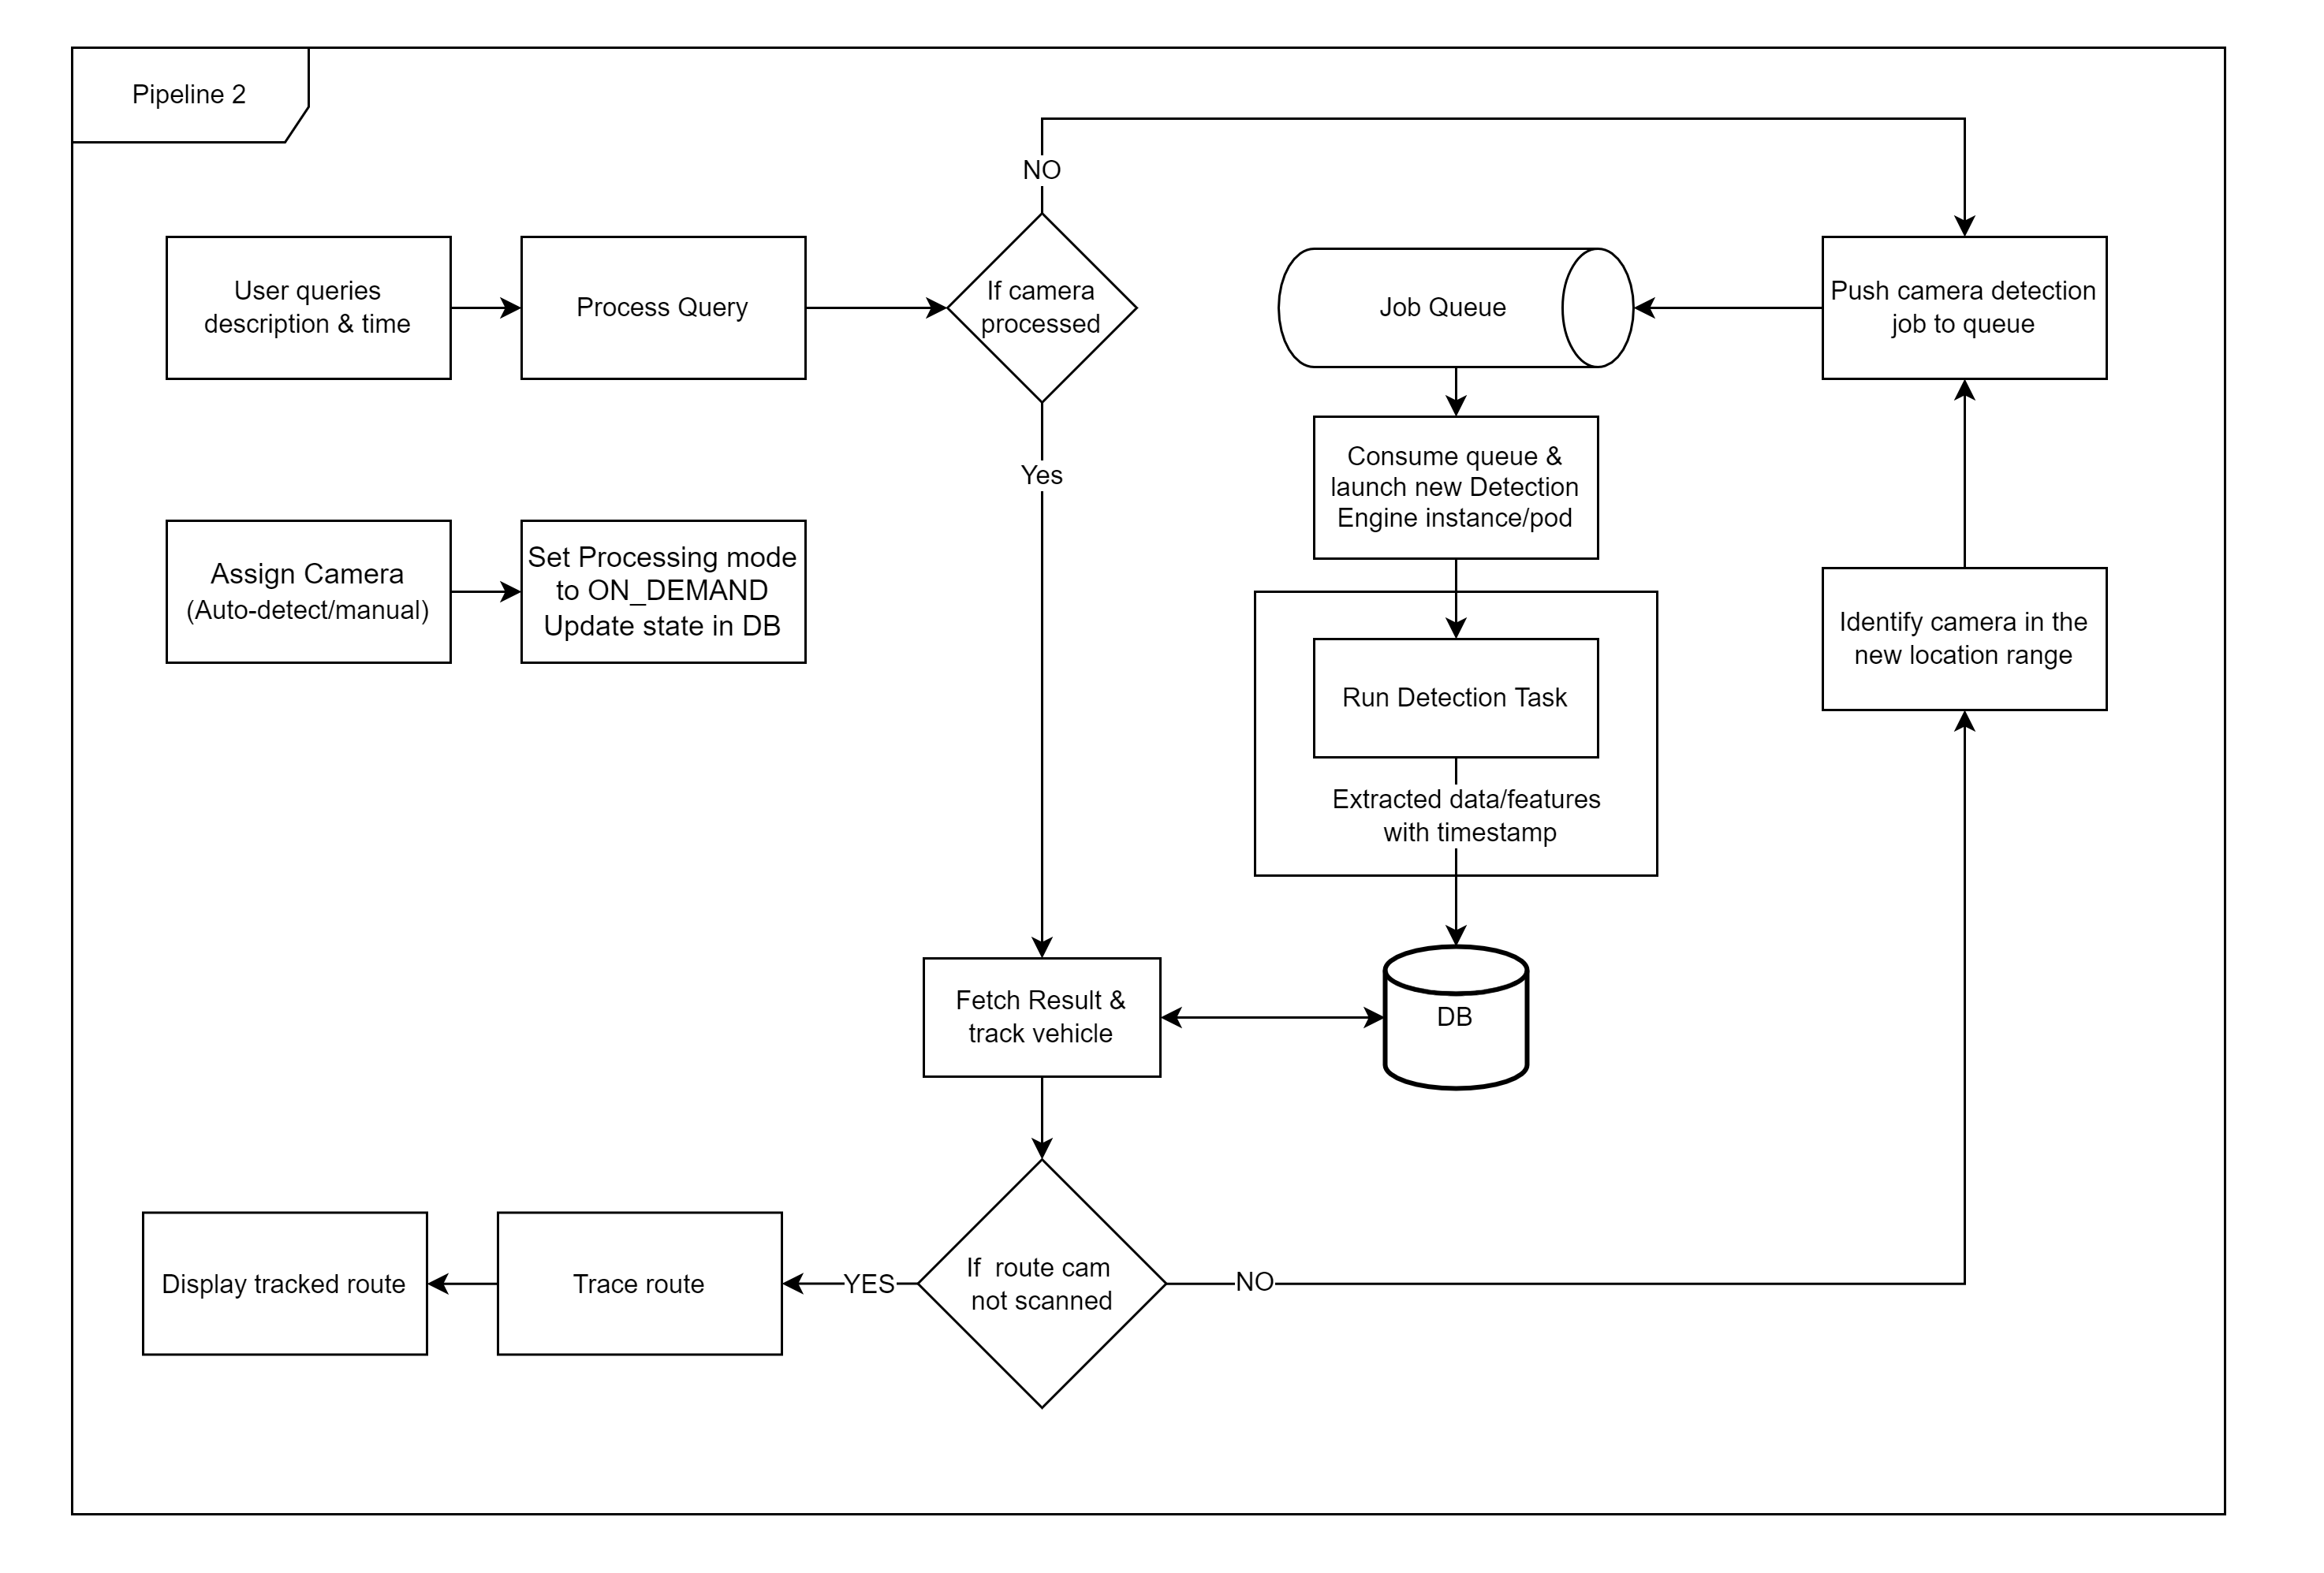
\includegraphics[width=\linewidth]{Images/pipeline2}
		\caption{pipeline2}
		\label{fig:pipeline2}
	\end{subfigure}
	\caption{Workflow pipeline}
\end{figure}

\lipsum[1]


\section{Camera Network}
The camera feed is obtained from a project deployed by Center for Information, Communication and Educational Technology (CICET), Government College of Engineering Kannur. Under the project entitled "Third eye", a virtual network was established covering an area of 350 $KM^2$, connecting 9 institutes. Using the existing cable network, various camera at installed allowing easy and secure storage and streaming. Currently the project houses holds about 190 cameras. Excess to these footage if obtained by secured virtual private junction.

\begin{figure}[!ht]
	\centering
	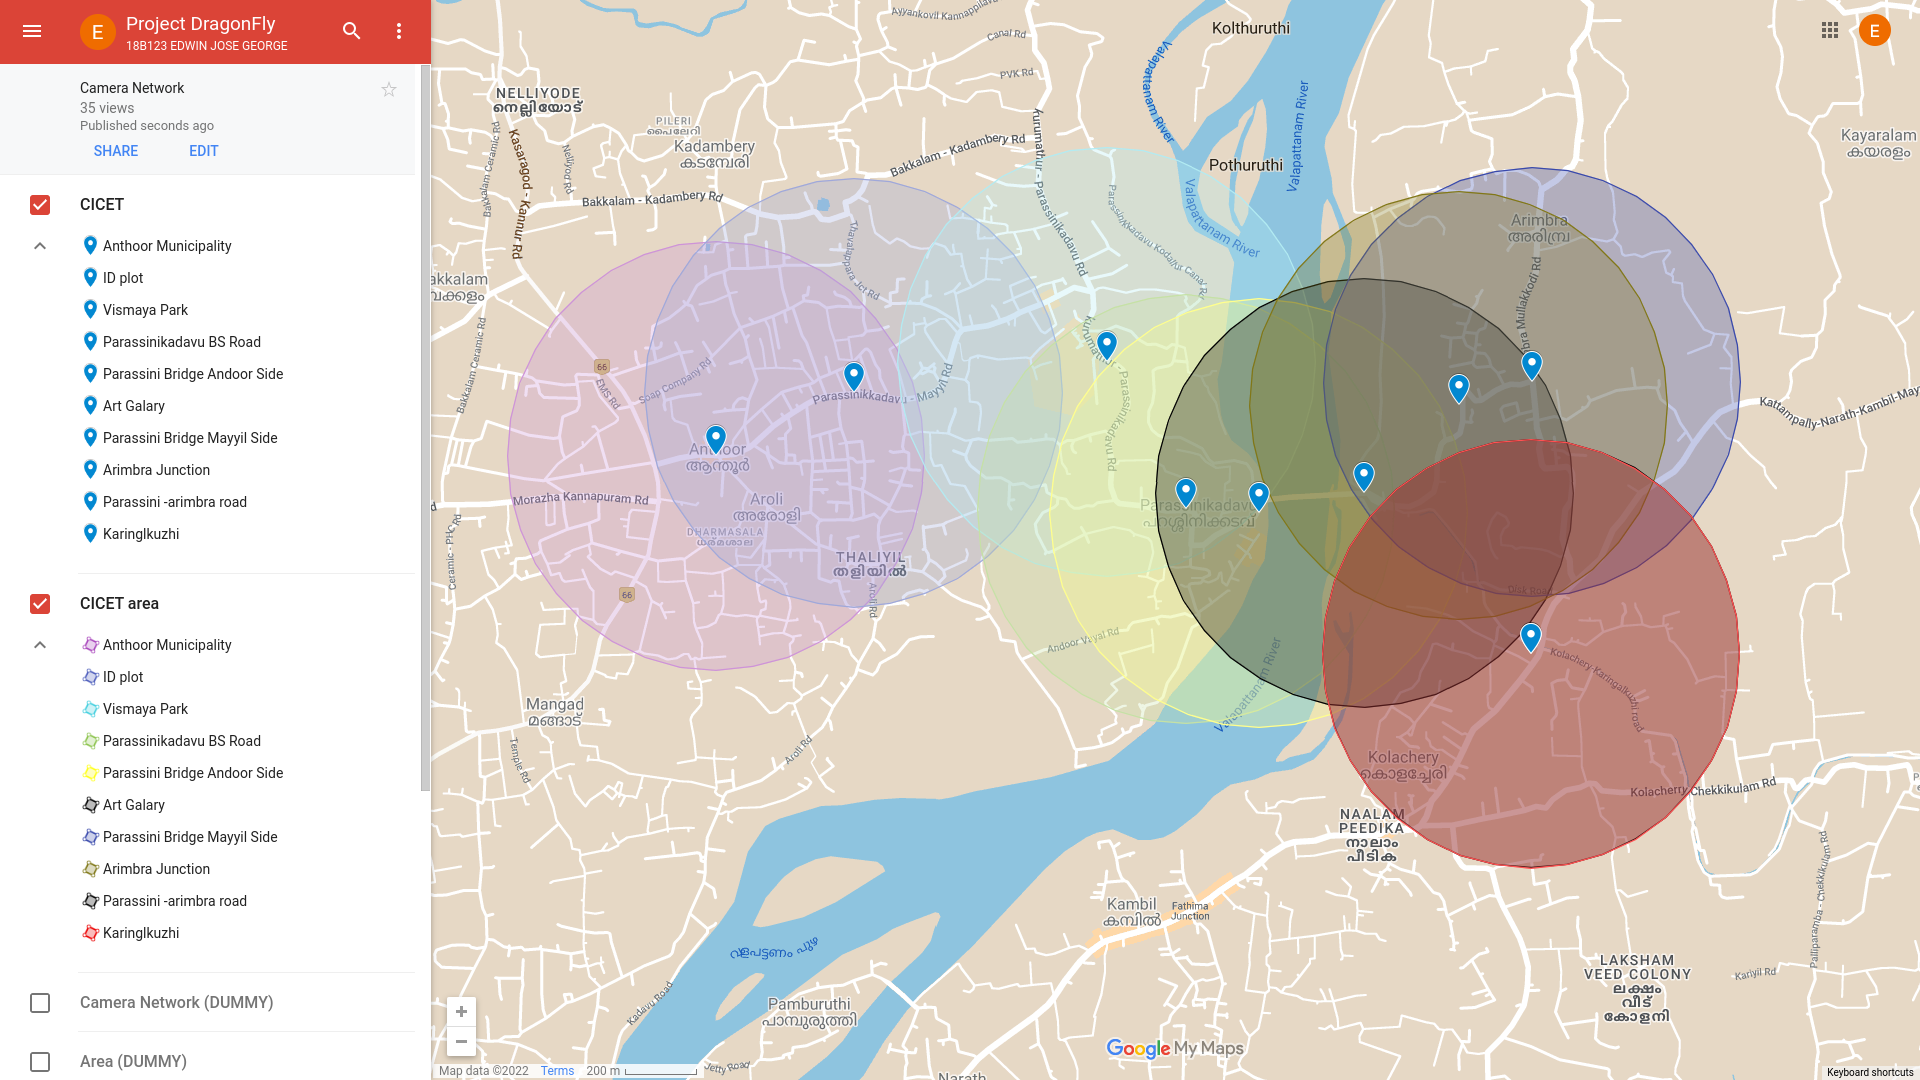
\includegraphics[width=\linewidth]{Images/camera-network}
	\caption{CICET camera network}
	\label{fig:camera-network}
\end{figure}

\begin{figure}[!ht]
	\centering
	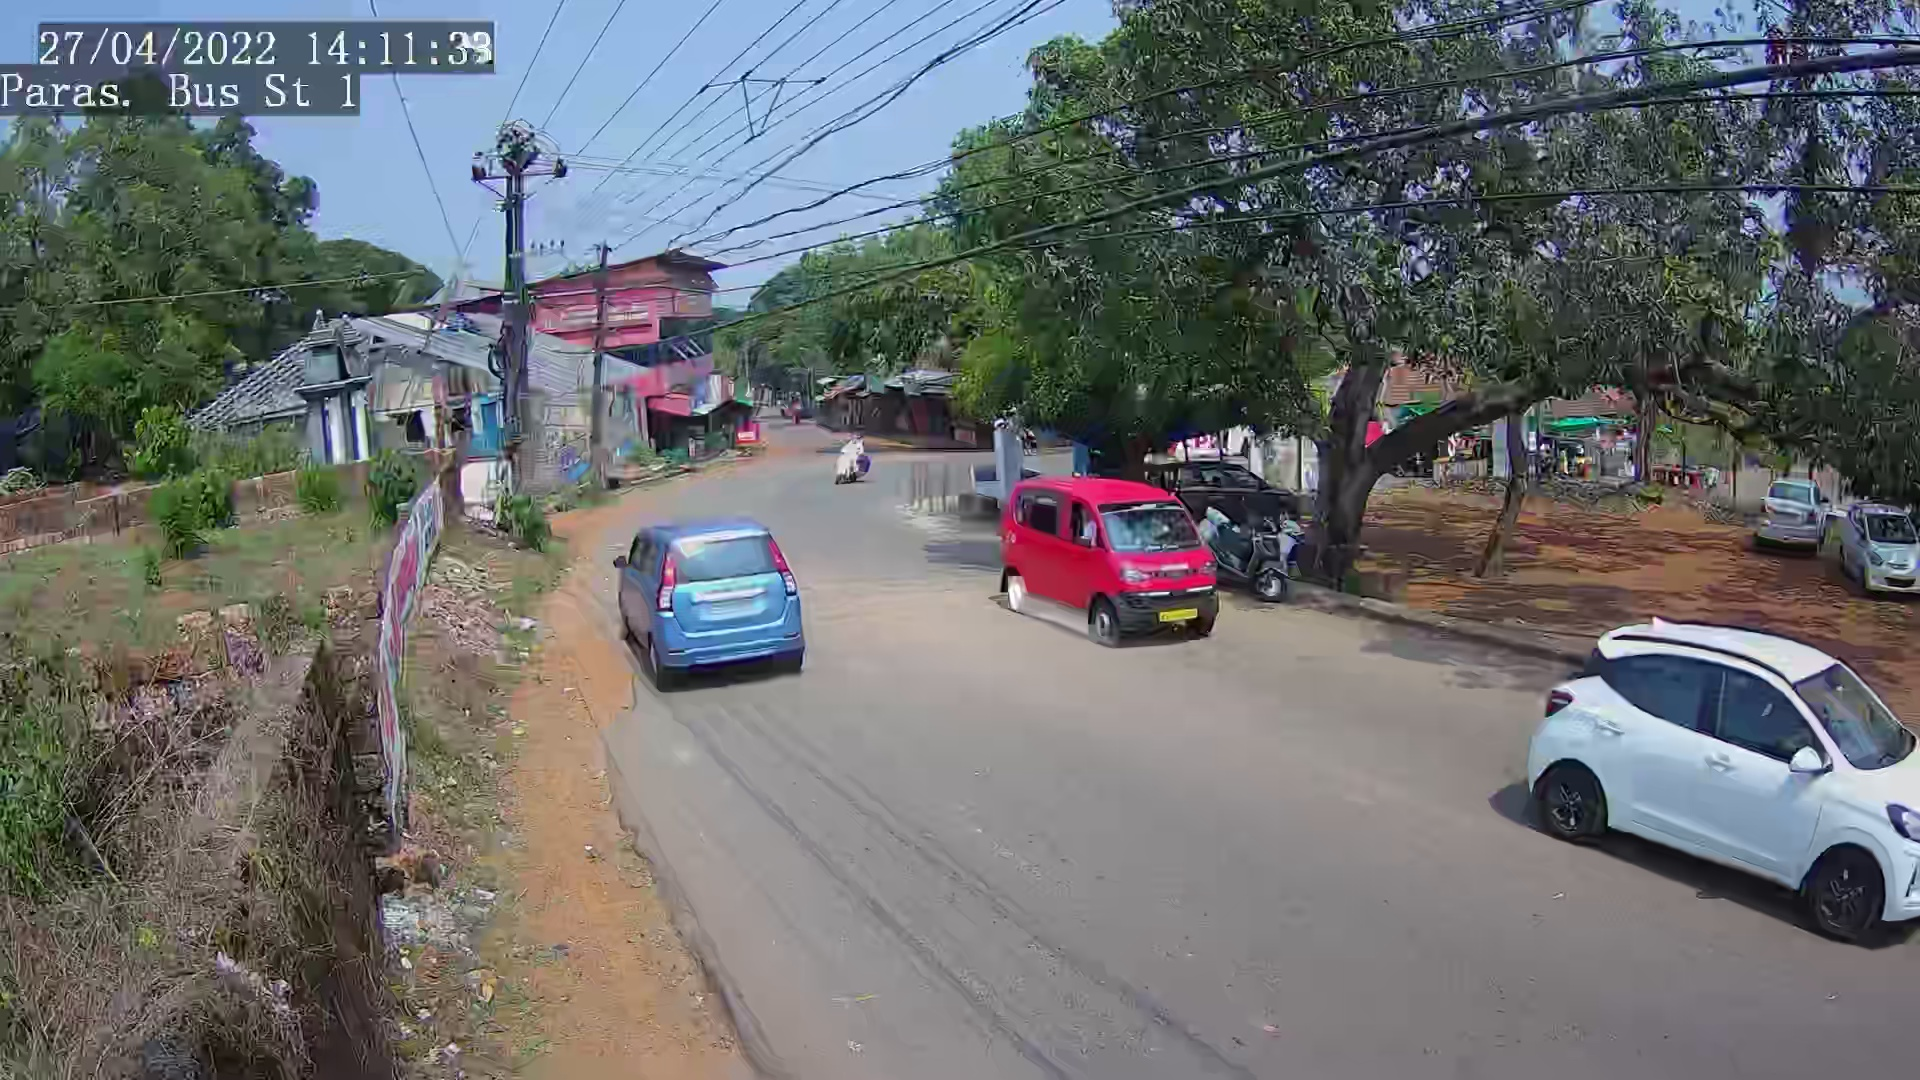
\includegraphics[width=0.32\linewidth]{Images/camera_footage/footage1} \hfill
	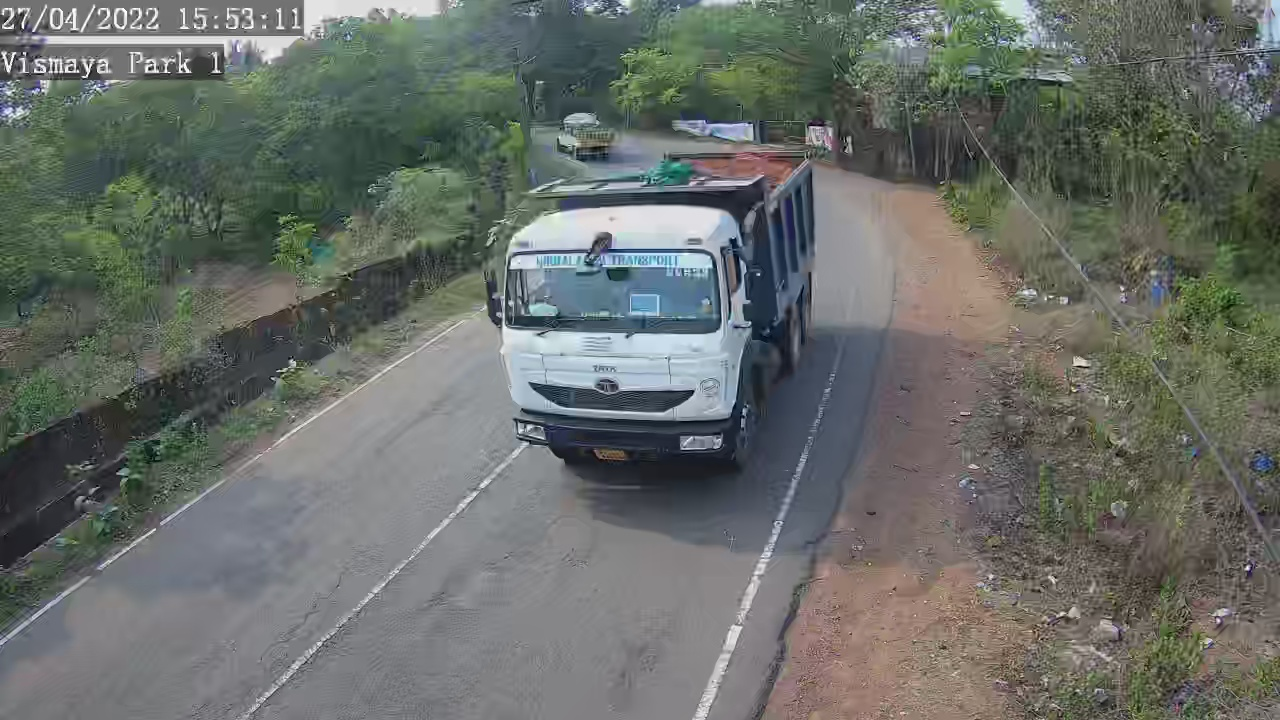
\includegraphics[width=0.32\linewidth]{Images/camera_footage/footage2} \hfill
%	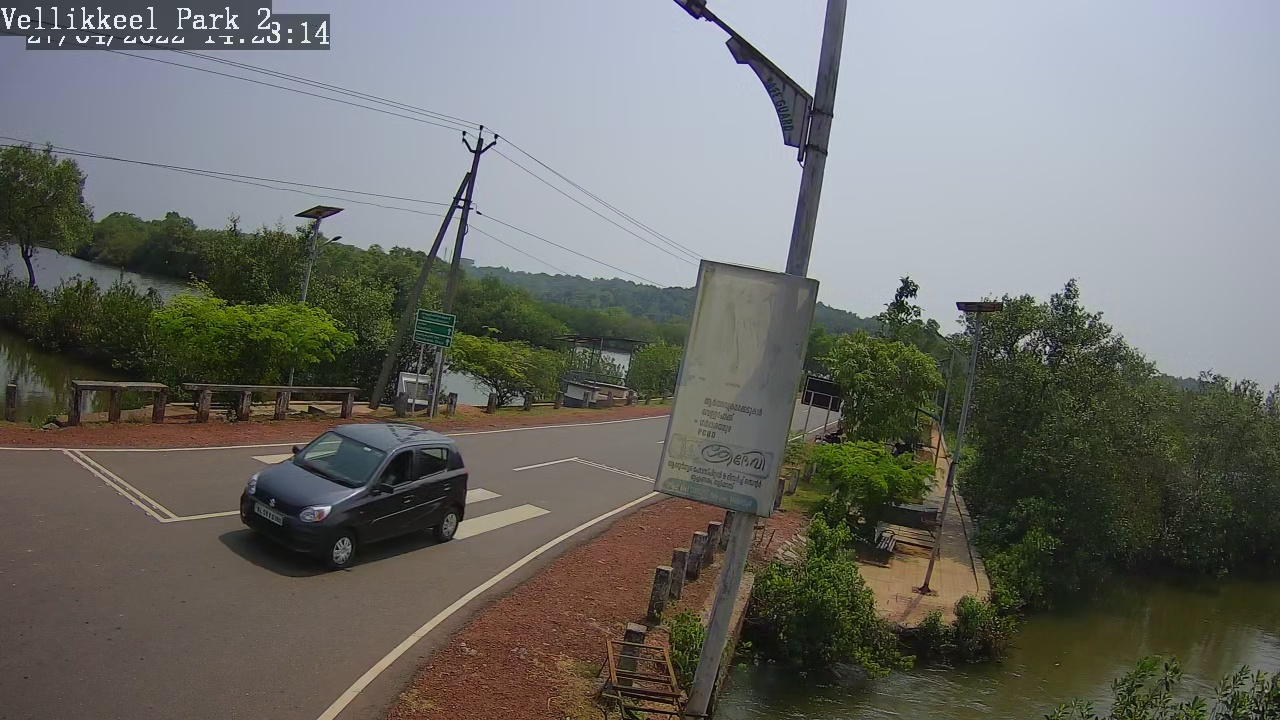
\includegraphics[width=0.32\linewidth]{Images/camera_footage/footage3} \\
%	\vspace{3mm}
%	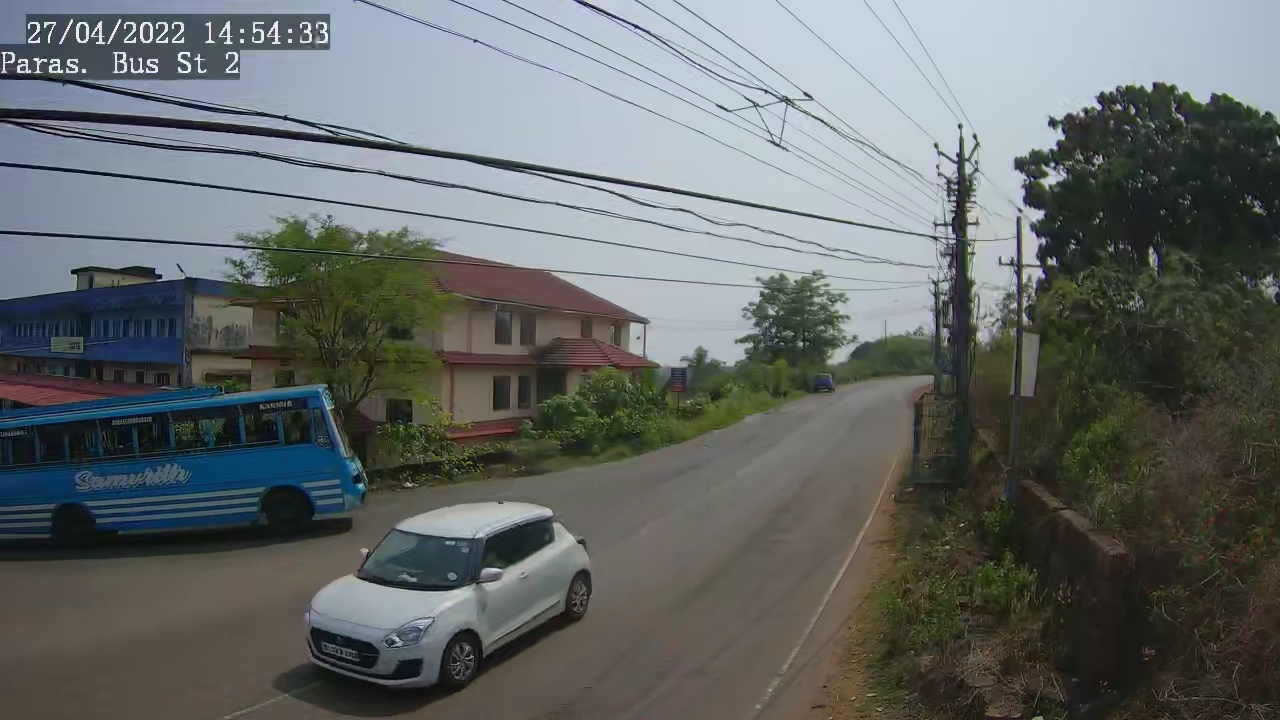
\includegraphics[width=0.32\linewidth]{Images/camera_footage/footage4} \hfill
	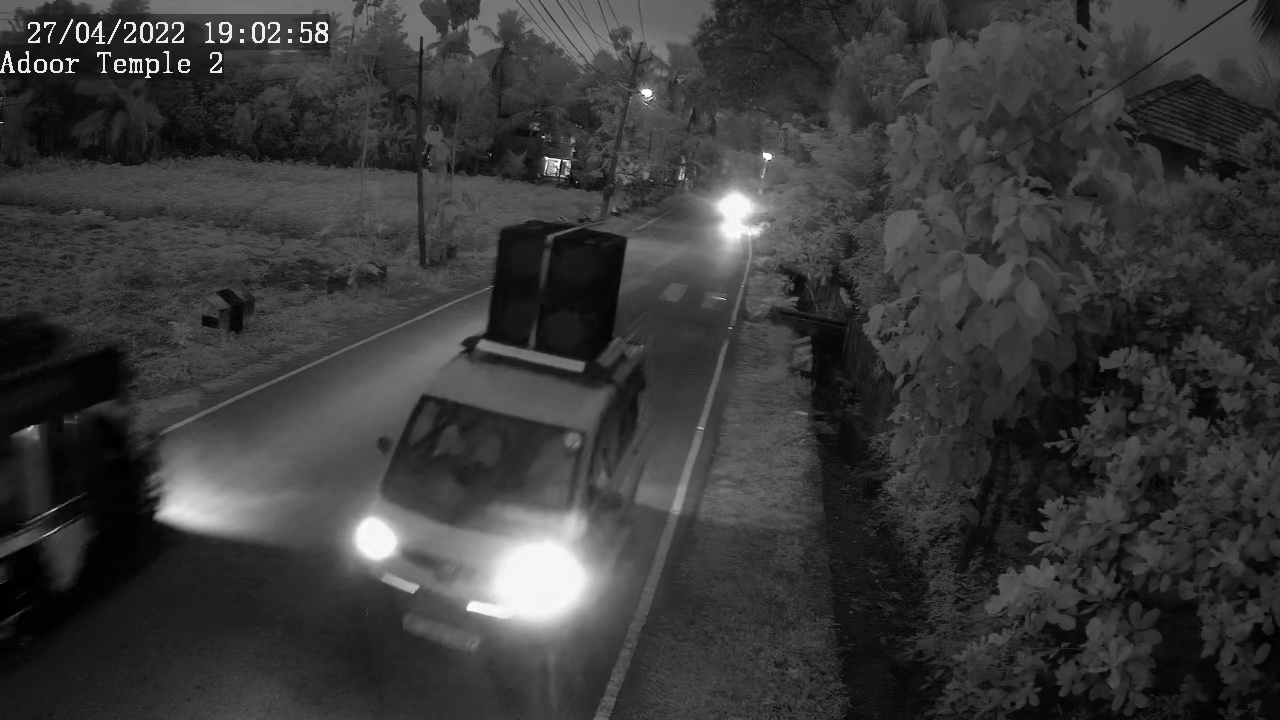
\includegraphics[width=0.32\linewidth]{Images/camera_footage/night1} \hfill
%	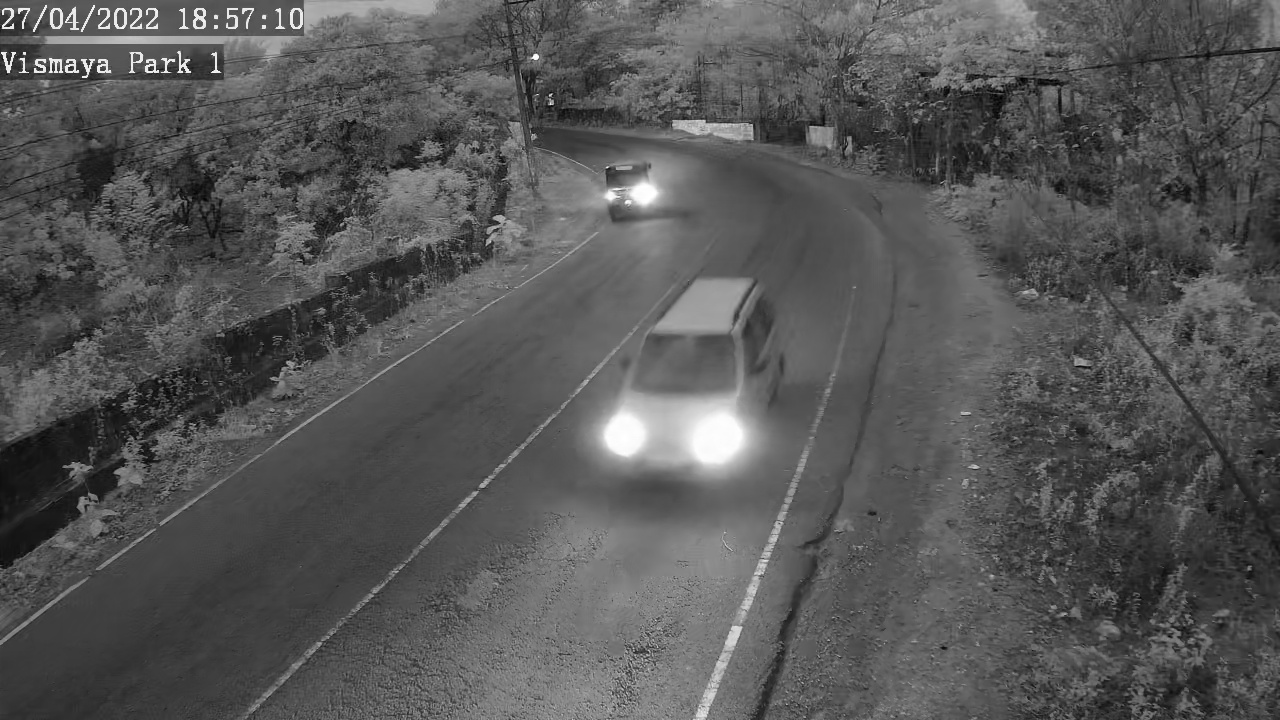
\includegraphics[width=0.32\linewidth]{Images/camera_footage/night2}
	\caption{Sample camera footage}
\end{figure}


\section{UI Design}
\lipsum[1]

\begin{figure}[!ht]
	\centering
	\begin{subfigure}[b]{0.48\linewidth}
		\centering
		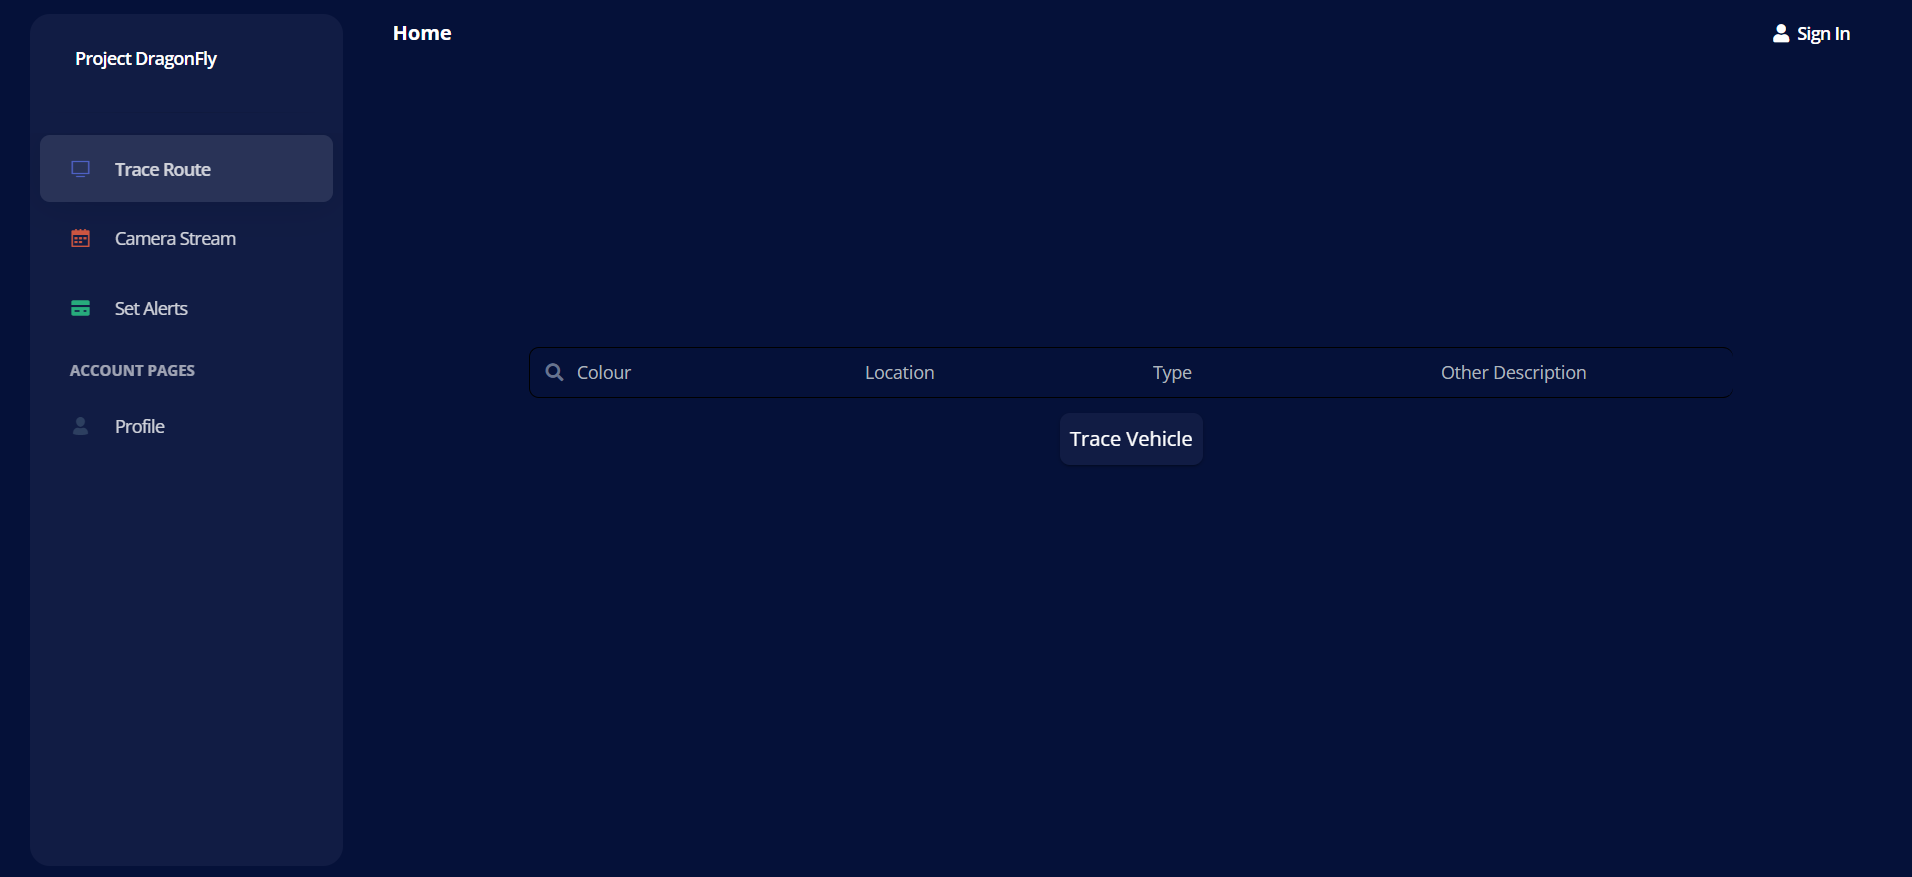
\includegraphics[width=\linewidth]{Images/UI/home}
		\caption{Home page}
		\label{fig:home}
	\end{subfigure} \hfill
	\begin{subfigure}[b]{0.48\linewidth}
		\centering
		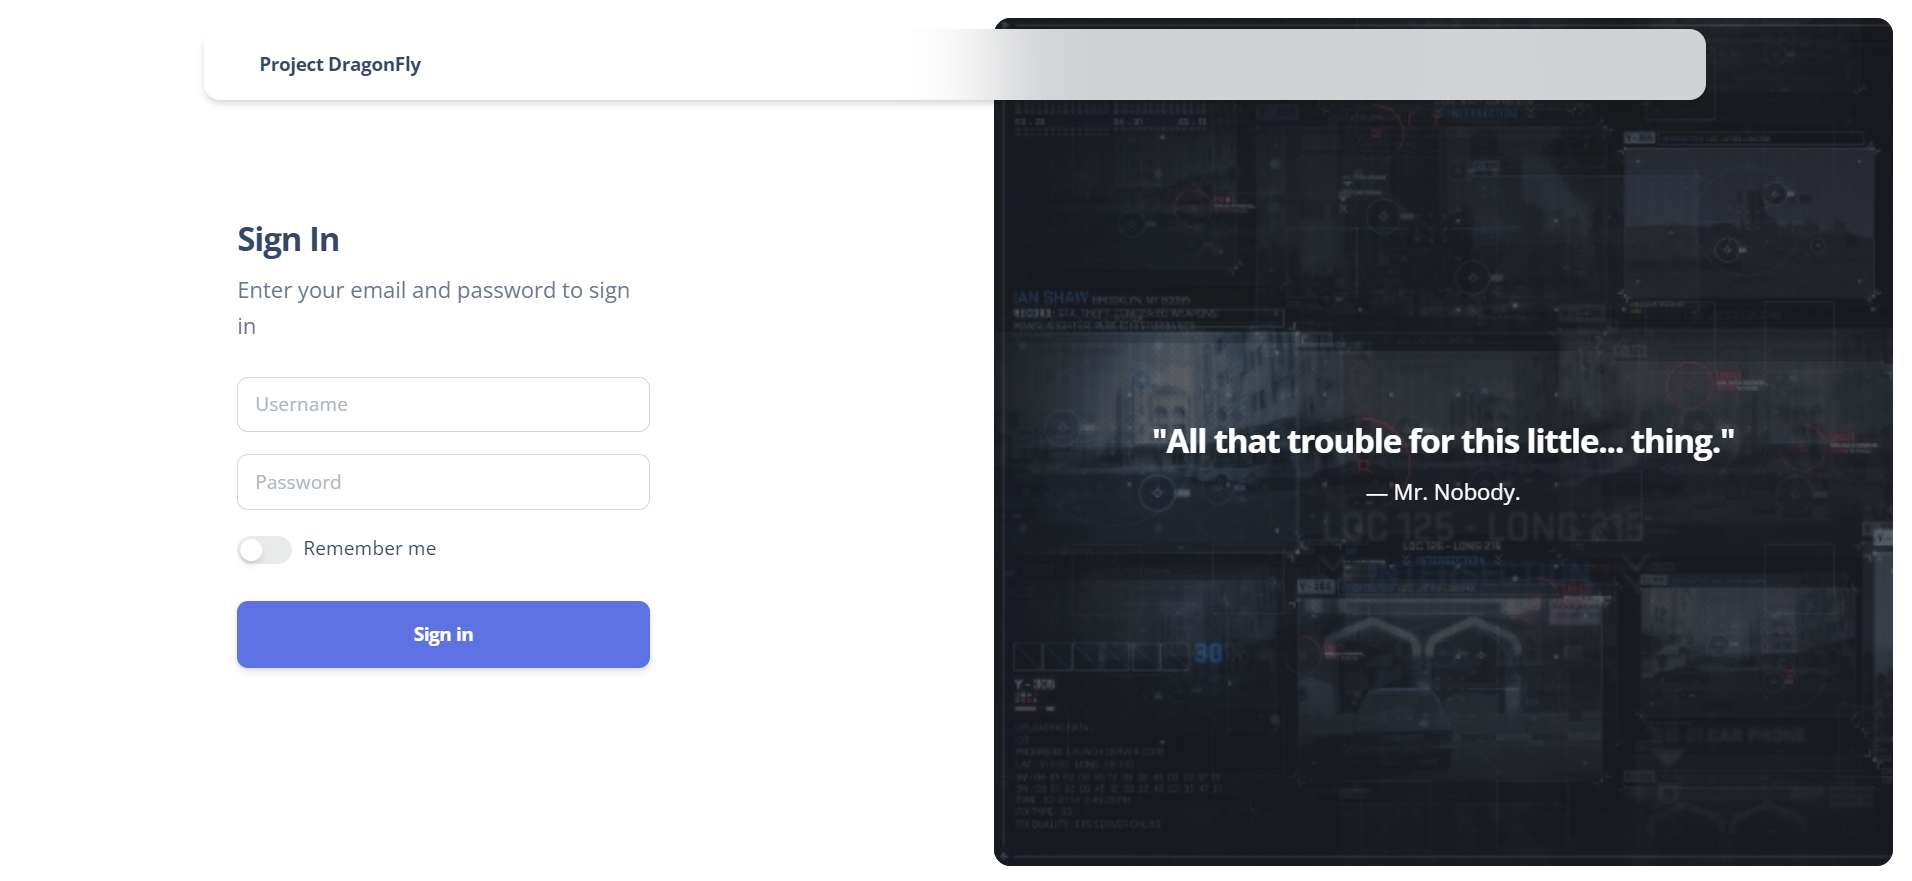
\includegraphics[width=\linewidth]{Images/UI/login}
		\caption{Login page}
		\label{fig:login}
	\end{subfigure} \\ \vspace{3mm}
	\begin{subfigure}[b]{0.48\linewidth}
		\centering
		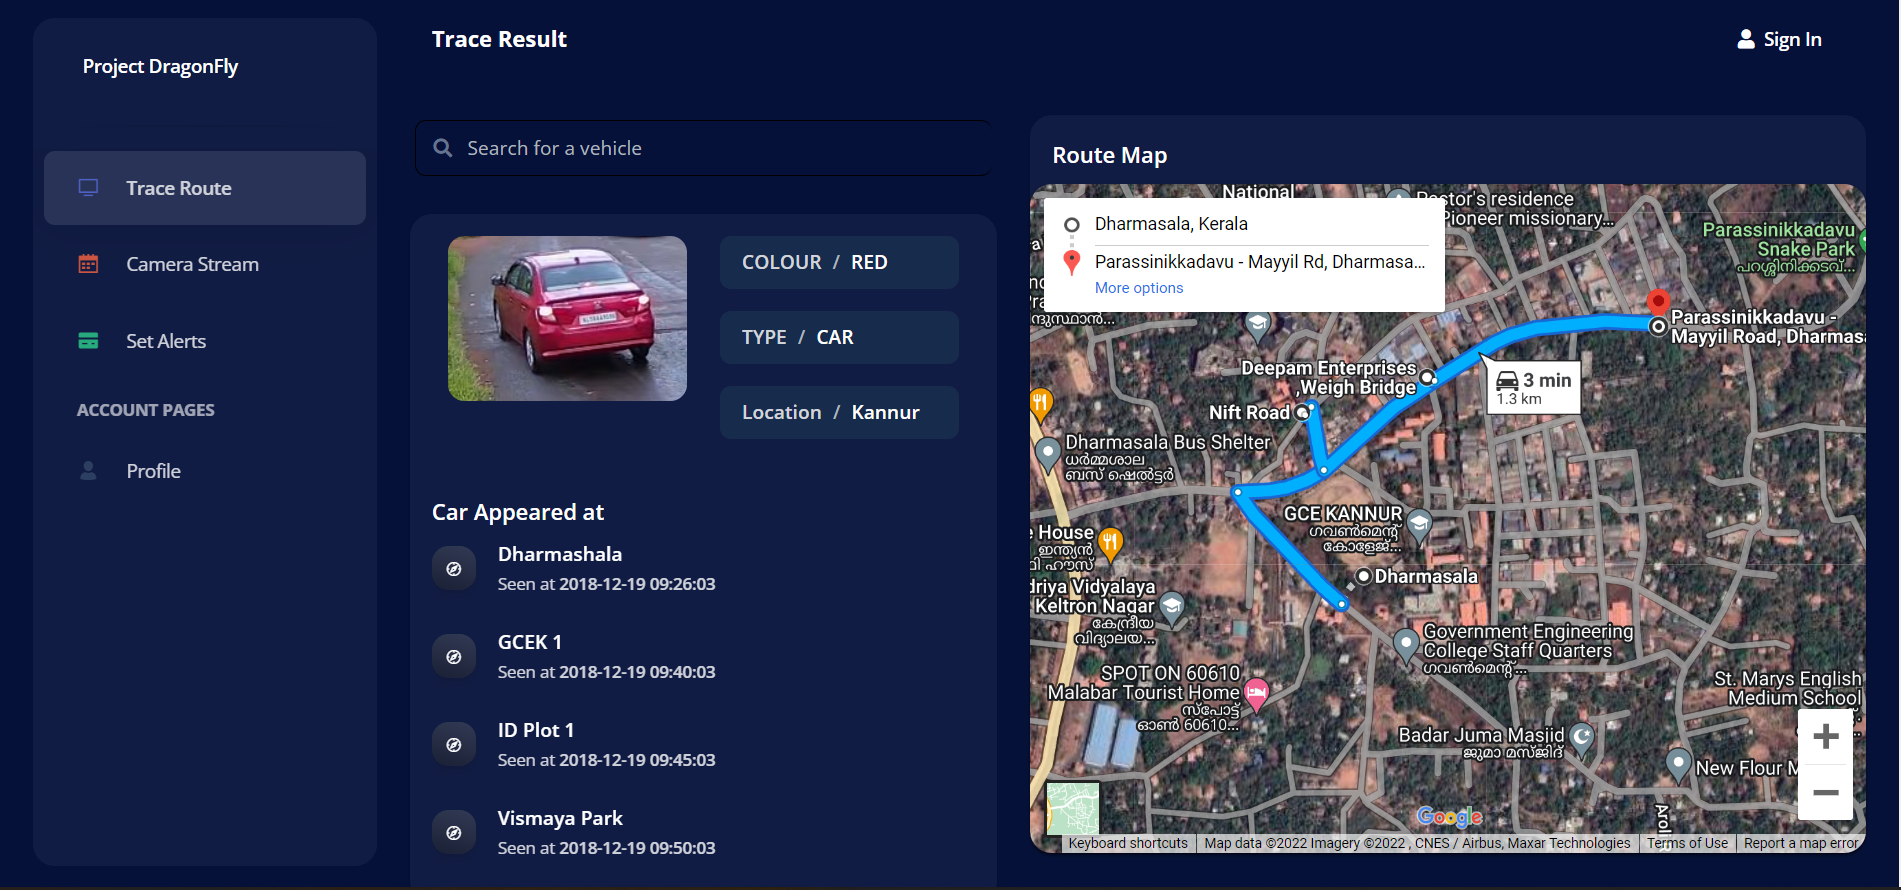
\includegraphics[width=\linewidth]{Images/UI/result}
		\caption{Result}
		\label{fig:result}
	\end{subfigure} \hfill
	\begin{subfigure}[b]{0.48\linewidth}
		\centering
		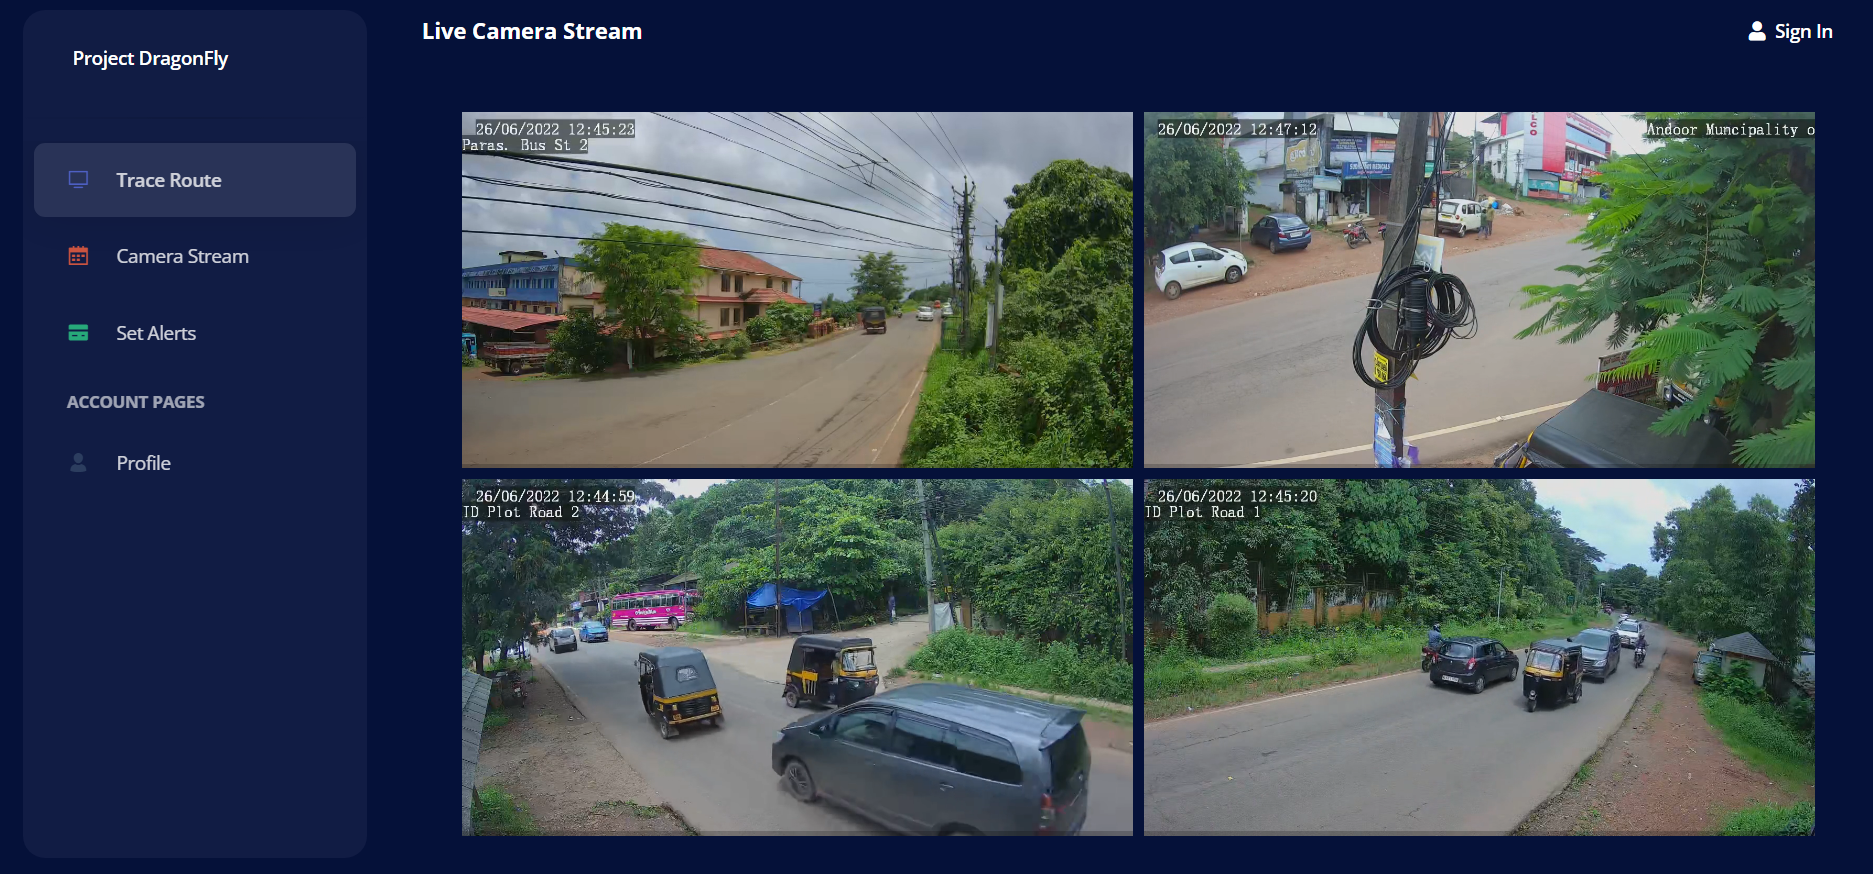
\includegraphics[width=\linewidth]{Images/UI/live_stream}
		\caption{Camera Live Stream}
		\label{fig:result}
	\end{subfigure} \hfill
	\begin{subfigure}[b]{0.48\linewidth}
		\centering
		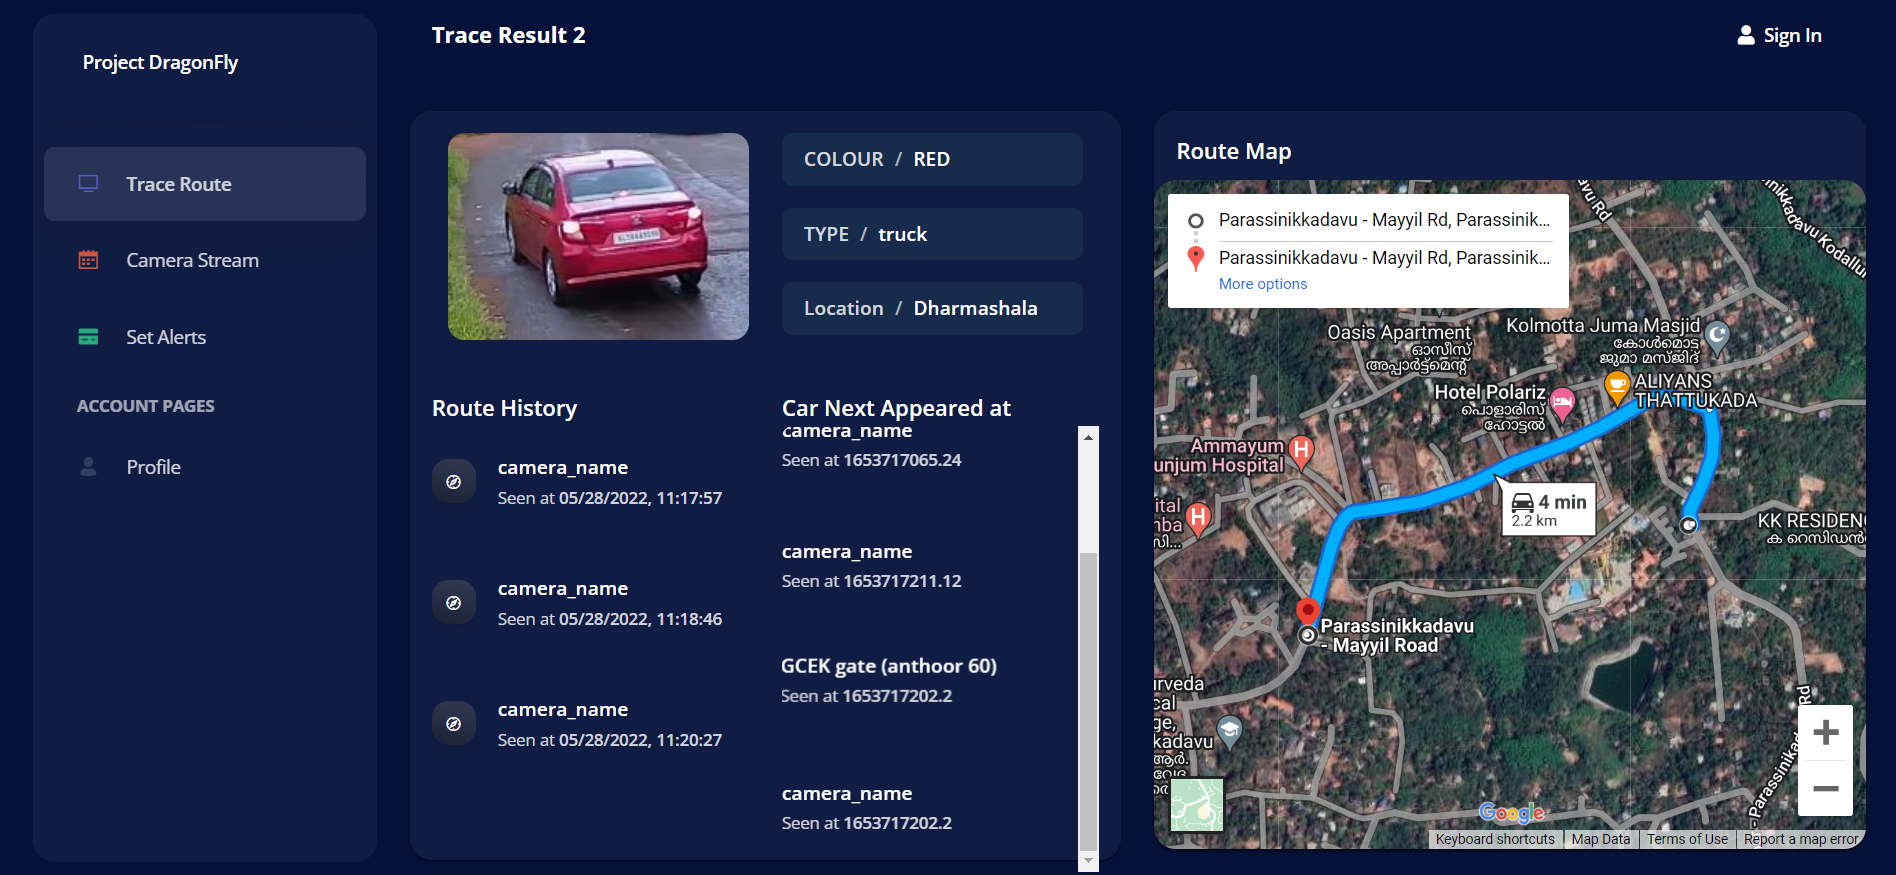
\includegraphics[width=\linewidth]{Images/UI/tracing}
		\caption{Tracing}
		\label{fig:tracing}
	\end{subfigure}
	\caption{UI Design}
\end{figure}

\section{AI Model}
\subsection*{YOLOv4}
YOLOv4 model is used for the detection of vehicles. Transfer learning was conducted on the AI model that significantly reduced the training time required. Transfer learning is the process of using a pre-trained model and changing its parameter to learn new/fine tuned concept. Pre-trained weight was extracted from the official YOLOv4 repository \cite{darknet} that used MS COCO dataset to train 80 classes. Parameter tuning is performed which are detailed in table \ref{tab:yolo_parameter}.

\begin{table}[!ht]
	\centering
	\begin{tabular}{|l|l|}
		\hline
		Input size            & $416 * 416$  \\ \hline
		Input Channels        & 3            \\ \hline
		Batch size            & 32           \\ \hline
		learning rate         & 0.0013       \\ \hline
		Yolo layer            & $[256*256],[512*512],[1024*1024]$ \\ \hline
		Total Layers          & 162          \\ \hline
		Target Classes (9)    & \begin{tabular}[c]{@{}l@{}}
			auto, bus, tempo traveler, tractor, \\
			truck, van, two wheeler, car, jcb\end{tabular} \\ \hline
	\end{tabular}%
	\caption{YOLOv4 Parameter}
	\label{tab:yolo_parameter}
\end{table}

The model was trained using Darknet at Google Colab. Later the environment was changed to the Workstation provided by the Dept. of Computer Science and Engineering, Govt. College of Engineering Kannur. A total of approx. 48 hours are spend in training, reaching 97.7\% mean Average Precision (mAP) at 7300 iterations. Figure \ref{fig:darknettrainingchart} summarizes training.

The dataset for training was collected at two different sources. Kaggle provided a wide variety of Indian Vehicle dataset that spanned across country. Footage from CICET camera network is also extracted. Each and every frame was labeled using LabelImg tool. Summary of the labeled dataset is depicted in the table \ref{tab:dataset_sum1}.

\begin{table}[!ht]
	\begin{tabular}{m{0.45\linewidth} m{0.45\linewidth}}
%		\begin{figure}
			\centering
			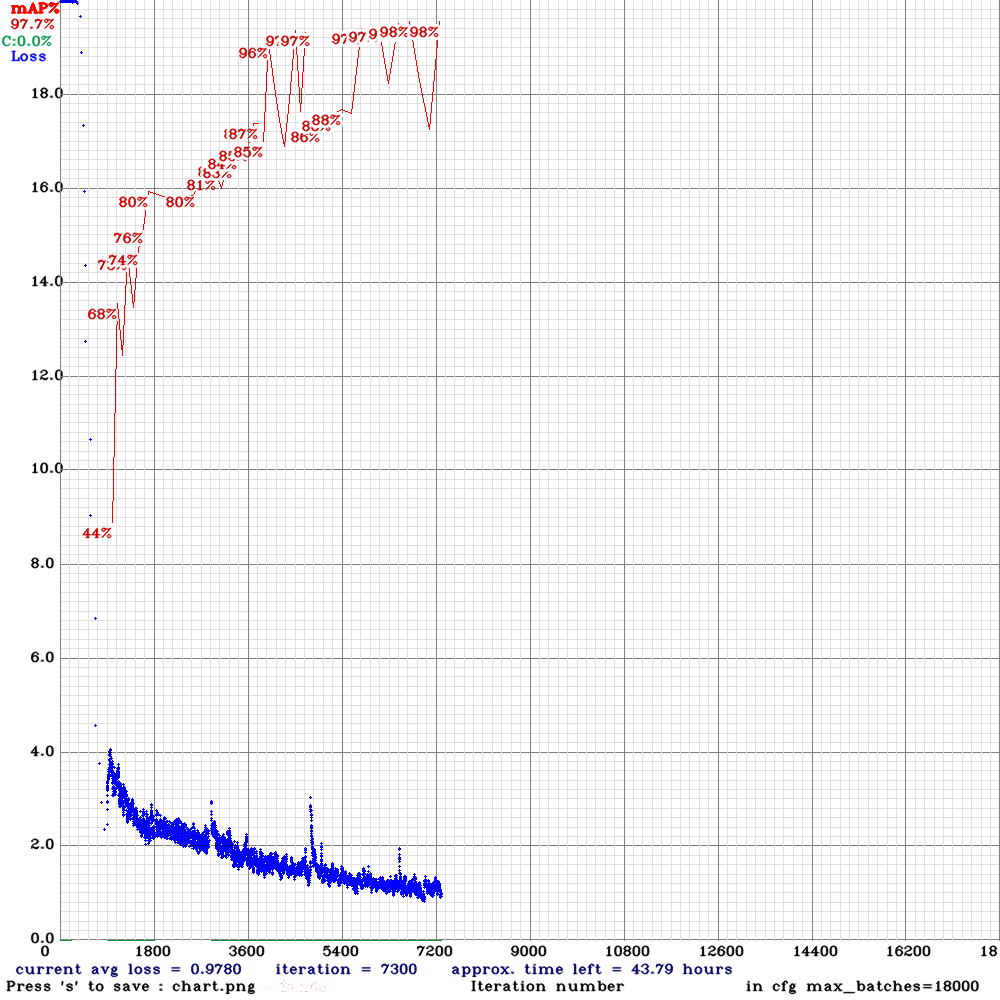
\includegraphics[width=\linewidth]{Images/darknet_training_chart}
			\captionof{figure}{YOLOv4 training chart}
			\label{fig:darknettrainingchart}			
%		\end{figure}

		 & 
		 
		 \begin{tabular}{|l|c|c||c|}
		 	\hline
		 	\textbf{Class}        & \textbf{Kaggle} & \textbf{CICET} & \textbf{Total} \\ \hline
		 	Two wheeler           & 557             & 291            & \textbf{848}   \\ \hline
		 	Truck                 & 354             & 170            & \textbf{424}   \\ \hline
		 	Auto                  & 297             & 146            & \textbf{443}   \\ \hline
		 	car                   & 233             & 432            & \textbf{665}   \\ \hline
		 	bus                   & 220             & 112            & \textbf{332}   \\ \hline
		 	tractor               & 133             & 0              & \textbf{113}   \\ \hline
		 	van                   & 101             & 131            & \textbf{232}   \\ \hline
		 	JCB                   & 1               & 0              & \textbf{1}     \\ \hline \hline
		 	\textbf{Total Boxes}  & \textbf{1956}   & \textbf{1282}  & \textbf{3238}  \\ \hline
		 	\textbf{Total Images} & \textbf{733}    & \textbf{826}   & \textbf{1559}  \\ \hline
		 \end{tabular}
		 \captionof{table}{Dataset summary}
		 \label{tab:dataset_sum1}
	\end{tabular}
\end{table}

\subsection*{DeepSORT}
DeepSORT is utilized to assign unique id to each object in an continuous frame. The implementation is directly extracted from the article of AIGuysCode \cite{theaiguyscode_deepsort}. The given model tries to extract human features as the deep matrix. No modification are made as Kalman filter provides greater accuracy. However, learning the deep matrix of vehicles can further increase accuracy and aid in siamese network.

\subsection{Image Dictionary}
In-order to facilitate correct labeling of images, a concept called Image Dictionary is introduced. Image Dictionary is a hierarchical classification of images. Each type can have its sub-type. A visual representation is also provided for each type. It is build using D3 JS.
\begin{figure}[H]
	\centering
	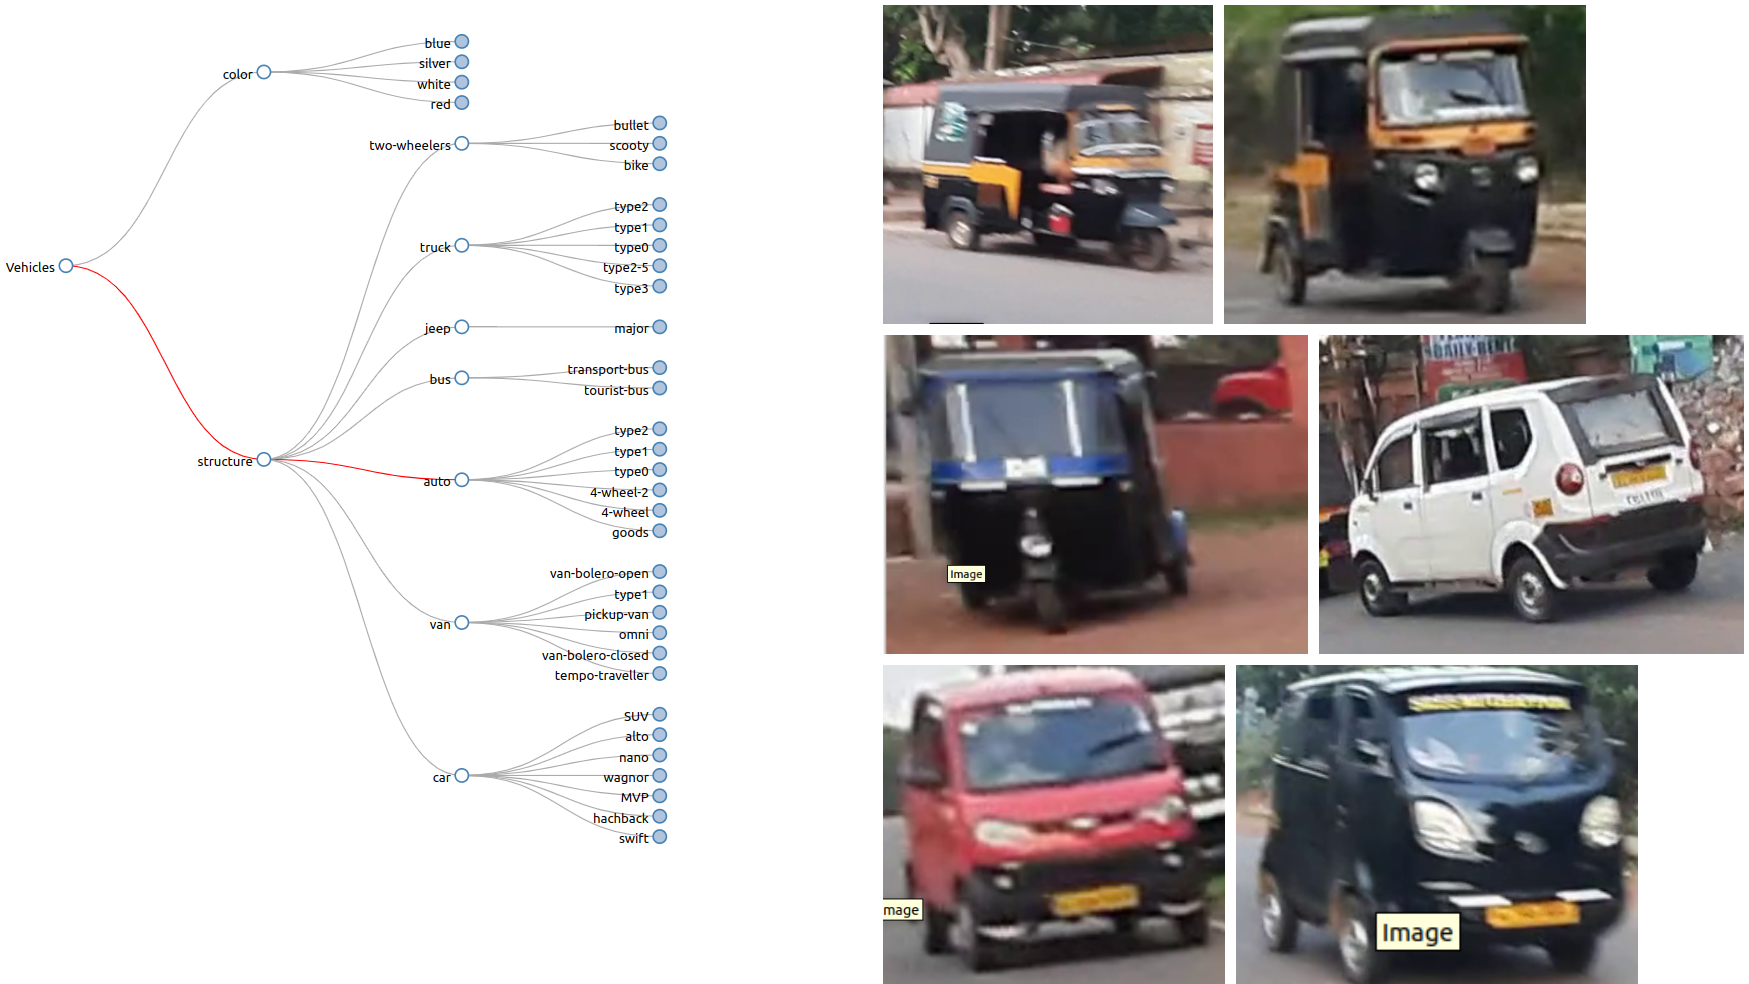
\includegraphics[width=\linewidth]{Images/image_dictionary}
	\caption{Image Dictionary}
\end{figure}


\section{Algorithm}
\begin{breakablealgorithm}
	\caption{Process and store detections $\forall$ camera}
	~~ \\\textbf{INPUT} : $video$, $camProp$
	\\ \textbf{OUTPUT} : $id$, $class$, $bbox$, $time$, $featureTensor$ $\rightarrow$ $Database$
	\begin{algorithmic}[1]
		\State $FPS \gets video.FPS$
		\State $time \gets camProp.startTime$
		\State $tracker \gets \Call{Tracker}{cosineMetric}$
		\ForAll{$frame \in video.frames$}
			\State $names, bboxes, scores \gets \Call{YOLOv4}{frame}$
			\State $features \gets \Call{encoder}{frame,bboxes}$ \Comment{feature extraction}
			\State $detections \gets []$
			\For{$i \in \Call{lenght}{names}$}
				\State $detections[i] \gets (names[i],bboxes[i],scores[i],features[i])$
			\EndFor
			\State $\Call{tracker.predict}{\space}$
			\State $\Call{tracker.update}{detections}$ \Comment{DeepSORT assigns id}
			
			\ForAll{$track \in tracker.tracks$}
				\If{$not \Call{track.isConfirmed}{\space}$} \Comment{Skip first few frame to ensure objects presence}
					\State Continue
				\ElsIf{$track.time_since_update \ge 1$} \Comment{Missing object in current frame}
					\State Continue
				\EndIf
				\State $\Call{Database.Write}{track.id, track.class, track.tbwh, time, track.feature}$
			\EndFor
			\State $time \gets time + \frac{1}{FPS}$
		\EndFor
	\end{algorithmic}
\end{breakablealgorithm}

\begin{breakablealgorithm}
	\caption{Route building}
	~~ \\\textbf{INPUT} : $vehicleClass$, $initialCamera$, $startTime$, $endTime$
	\\ \textbf{OUTPUT} : $route$
	\begin{algorithmic}[1]	
		\State $terminate \gets FALSE$
		\State $route \gets []$
		\State $vehicleList \gets []$
		\State $currentCam \gets initialCamera$
		
		\State $DB \gets currentCam.DataBase$  \Comment{Find the vehicle}
		\State $DB \gets \Call{DB.filter}{name=vehicleClass}$
		\State $fDB \gets \Call{DB.filter}{time \geq startTime}$
		\State $fDB \gets \Call{fDB.filter}{time \leq endTime}$
		
		\ForAll{ $vid \in \Call{uniqueID}{fDB}$}
			\State $vDB \gets \Call{DB.filter}{id = vid}$
			\State $enterTime \gets \Call{min}{vDB.time}$
			\State $exitTime \gets \Call{max}{vDB.time}$
			\State $\Call{vehicleList.append}{vid,enterTime,exitTime,currentCam}$
		\EndFor
		
		\While{$terminate \neq FALSE$}	\Comment{Search route iteratively}
			\If{$\Call{count}{vehicleList} == 0$}
				\State $terminate \gets TRUE$
				\State Break
			\ElsIf{$\Call{count}{vehicleList} == 1$}
				\State $seletedVehicle \gets vehicleList[0]$
			\Else
				\State $selectedVehicle \gets \Call{UserSelect}{vehicleList}$
			\EndIf
			\State $\Call{route.append}{selectedVehicle}$ \Comment{Add to route list}
			
			\State $addedCam \gets selectedVehicle.camera$
			\State $nextCameras \gets \Call{addedCam.neighbor}{radius=1KM}$
			\State $vehicleList \gets []$
			

			\For{$currentCam \in nextCameras$}
				\State $startTime \gets selectedVehicle.exitTime + \Call{minTravelTime}{addedCam,currentCam}$
				\State $endTime \gets selectedVehicle.exitTime + \Call{maxTravelTime}{addedCam,currentCam}$
							
				\State $DB \gets currentCam.DataBase$  \Comment{Find the vehicles}
				\State $DB \gets \Call{DB.filter}{name=vehicleClass}$
				\State $fDB \gets \Call{DB.filter}{time \geq startTime}$
				\State $fDB \gets \Call{fDB.filter}{time \leq endTime}$
				
				\ForAll{ $vid \in \Call{uniqueID}{fDB}$}
					\State $vDB \gets \Call{DB.filter}{id = vid}$
					\State $enterTime \gets \Call{min}{vDB.time}$
					\State $exitTime \gets \Call{max}{vDB.time}$
					\State $\Call{vehicleList.append}{vid,enterTime,exitTime,currentCam}$
				\EndFor	
			\EndFor
		\EndWhile
		\State \Call{print}{route} \Comment{The final result}
	\end{algorithmic}
\end{breakablealgorithm}